% LaTeX Template for Project Report, Version 2.0
% (Abstracted from a Major Project Report at CSED, NIT Calicut but can be
% modified easily to use for other reports also.)
%
% Released under Creative Commons Attribution license (CC-BY)
% Info: http://creativecommons.org/licenses/by/3.0/
%
% Created by: Kartik Singhal
% BTech CSE Batch of 2009-13
% NIT Calicut
% Contact Info: kartiksinghal@gmail.com
%
% It is advisable to learn the basics of LaTeX before using this template.
% A good resource to start with is http://en.wikibooks.org/wiki/LaTeX/
%
% All template fields are marked with a pair of angular brackets e.g. <title here>
% except for the ones defining citation names in ref.tex.
%
% Empty space after chapter/section/subsection titles can be used to insert text.
%
% Just compile this file using pdflatex after making all required changes.

\documentclass[12pt,a4paper]{report}
\usepackage[pdftex]{graphicx} %for embedding images
\usepackage{url} %for proper url entries
\usepackage[bookmarks, colorlinks=false, pdfborder={0 0 0}, pdftitle={<pdf title here>}, pdfauthor={<author's name here>}, pdfsubject={<subject here>}, pdfkeywords={<keywords here>}]{hyperref} %for creating links in the pdf version and other additional pdf attributes, no effect on the printed document
%\usepackage[final]{pdfpages} %for embedding another pdf, remove if not required

\begin{document}
\renewcommand\bibname{References} %Renames "Bibliography" to "References" on ref page

%include other pages
\begin{titlepage}

\begin{center}

\textup{\small {\bf MSA 8389 Directed Reading} }\\[0.2in]

% Title
\Large \textbf {Industry Trajectory Analysis}\\[0.5in]

\vfill

% Submitted by
\normalsize Submitted by \\
\begin{table}[h]
\centering
\begin{tabular}{lr}
Professor Peter Molnar \\ 
Abraham Hardy \\ 
\end{tabular}
\end{table}


\vfill

% Bottom of the page

\includegraphics[width=0.18\textwidth]{./gsu_bw}\\[0.1in]
\Large{Institute for Insight}\\
\normalsize
\textsc{Robinson College of Business}\\
Atlanta, Georgia\\
\vspace{0.2cm}
Fall Semester 2018

\end{center}

\end{titlepage}

\vspace{2in}
\begin{abstract}

Predicting trends and movements within a given industry sector can be an incredibly difficult, time consuming and potentially fruitless endeavor. The goal of the research conducted over this semester is to show the potential to use data analysis and eventually machine learning techniques to protect changes within a given industry. Python was used to pull information from the Wharton database the most connected companies were determined using graphing methods. Once the companies were selected a set of variables were compiled to represent how well a company was doing. The variables were standardized and PCA reduction was used to reduce the variables to two principle components. Once the graphs were completed, companies were grouped by sector to establish if any similarities existed between sectors. Several sectors had graphes with similar changes in trajectory. Upon looking at the events surronding changes it trajectory it was discovered that each change in trajectory on the graph corresponded to a major event affecting the company. Each of the companies narrtives have been examined to be the basis for moving from a descriptive model to the ultimate goal of predictive model of industry forces.
\end{abstract} 


\pagenumbering{roman} %numbering before main content starts
\tableofcontents


\newpage
\pagenumbering{arabic} %reset numbering to normal for the main content


\chapter{Indstrusy Research}

\section{Introduction}

	The research began by looking at the supply chain database created by Wharton. This database contained a list of companies and who they supplied to organized by year using the unique identifier gvkey. Using the gvkeys of the supplier as the source and the gvkeys of customers as destinations a directed graph was created to determine the most connected companies for each year. Throughout the years several companies appeared over and over. 
\section{Process}

	This small group of regularly highly connected companies became the base group for our research. Twenty-seven companies were divided into nine sectors: Automotive, Retail, Oil, Computers, Hardware, Telecommunication and Conglomerates. Several variables were selected to represent how well the companies were doing. Some of the variables included were total assets, net income, total sales and stock holder equity.\\
\newline

	Once the variables were compiled, they were standardized and a PCA reduction was performed. This allowed all twenty-seven companies to be compared side by side. Trends were noticed immediately regarding General Motors and Ford Motor Company. Once the selected companies were divided into smaller graphs, still using the original standardization and PCA from the large graph, more trends were noticed. \\
\newline

	One of the most striking trends within in an industry was the similarities between Home Depot and Lowe’s. The graphs had similar trajectories and then both changed trajectories in the same direction around the same time and then once again changed back to the original direction at the same time. Both changes in direction coincide with the begin and end of the house market crash. The oil industry has a whole has a lot of similar trajectories in the graphs for each of the companies, most noticeably between Exxon and Shell. \\
\newline

	As research began into the history of each of the companies and the events transpiring during each of the changes in trajectory one major theme occurred over and over. Nearly every change in a company’s trajectory coincided with a major event for the company. From the housing market crash in the hardware industry to AT\&T being bought by what was at the time a spin off company to the oil industry reacting to the changes in oil prices in the mid 2000’s.\\
\newline

	The discovery of the changes in graph trajectories has led to an increased emphasis on telling the story of each company.  The following sections of this paper are narratives of the major changes in each company’s graph and how those changes are representative of major events affect each company. \\
\chapter{Narratives}
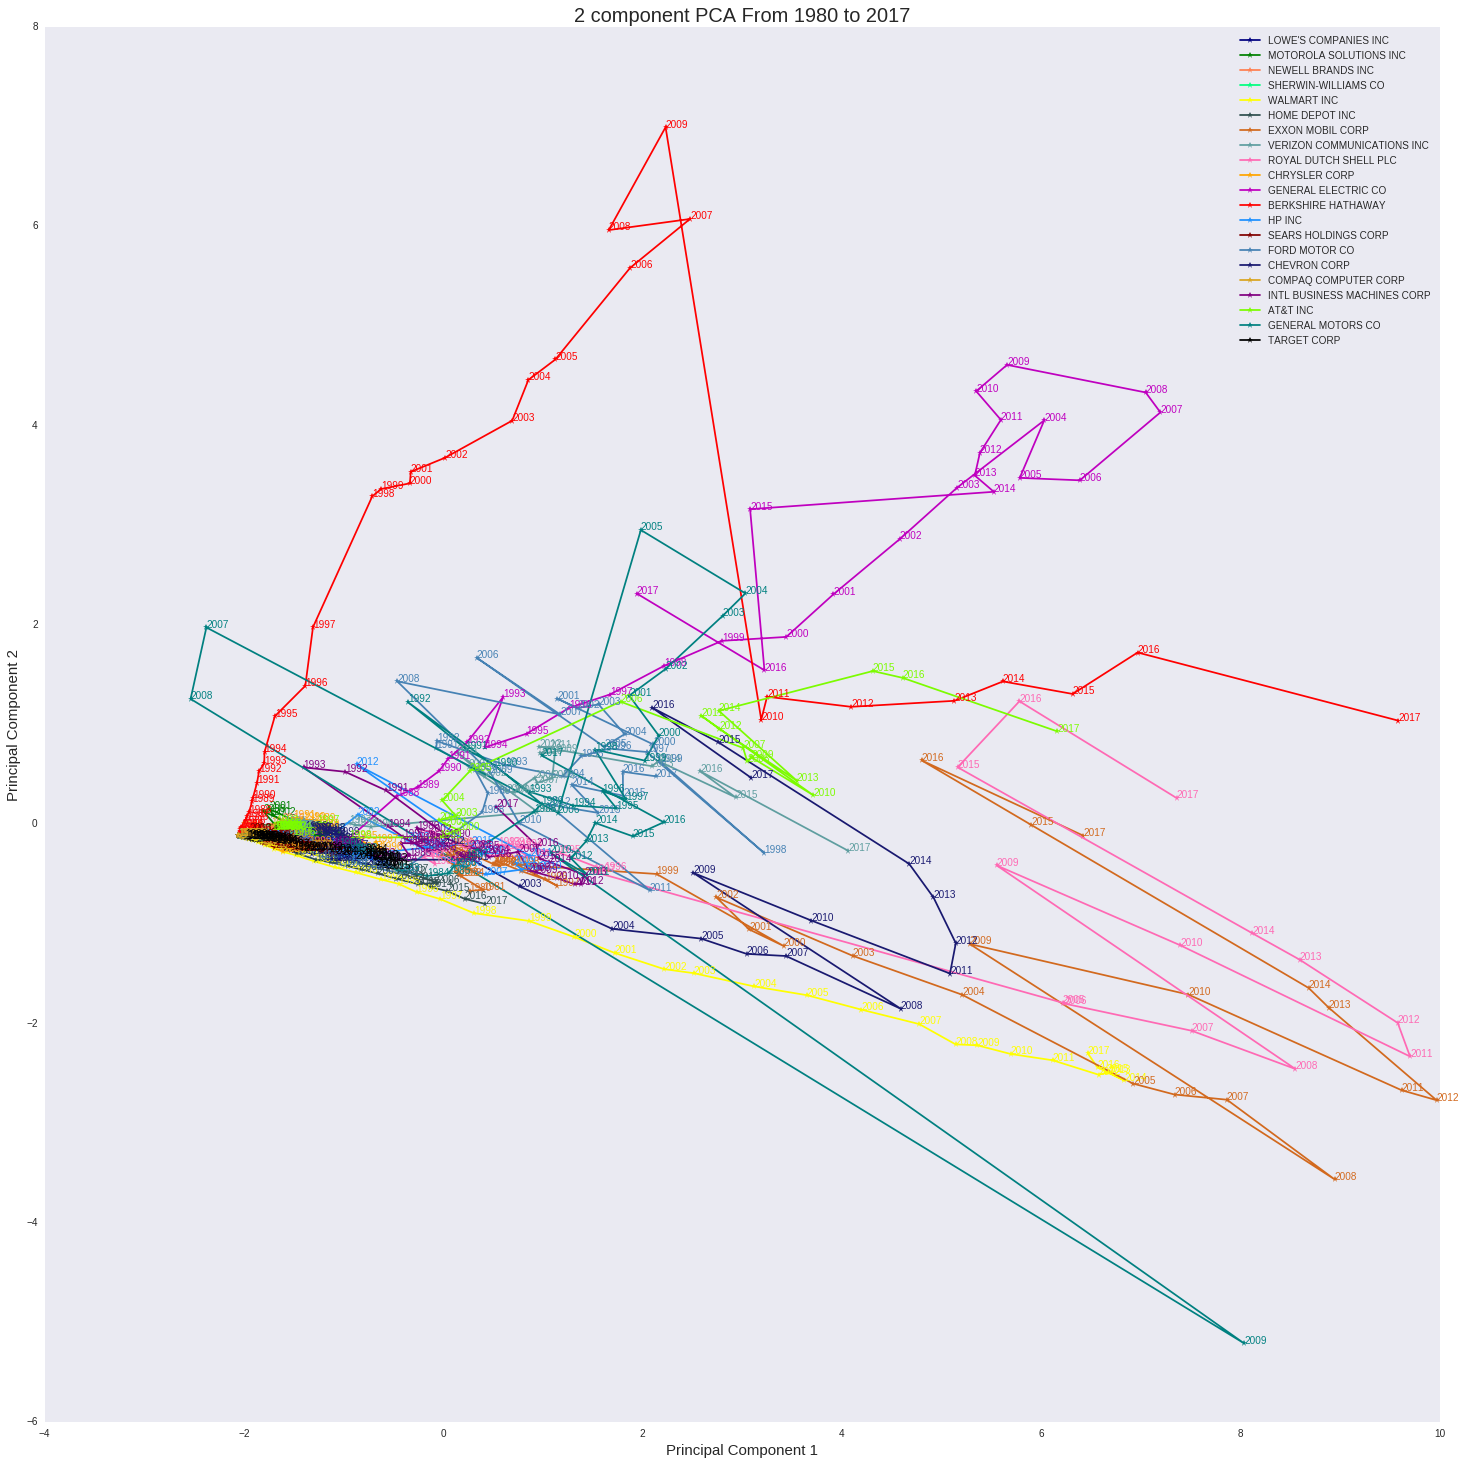
\includegraphics[width=1\textwidth]{./Main_Graph}\\[0.1in] \\

Several trends can be seen int the main graph such as Shell and Exxon or Lowes and Home Depot. Each of these indivisual graphes will be broken down more throughout this section.

\section{Hardware}
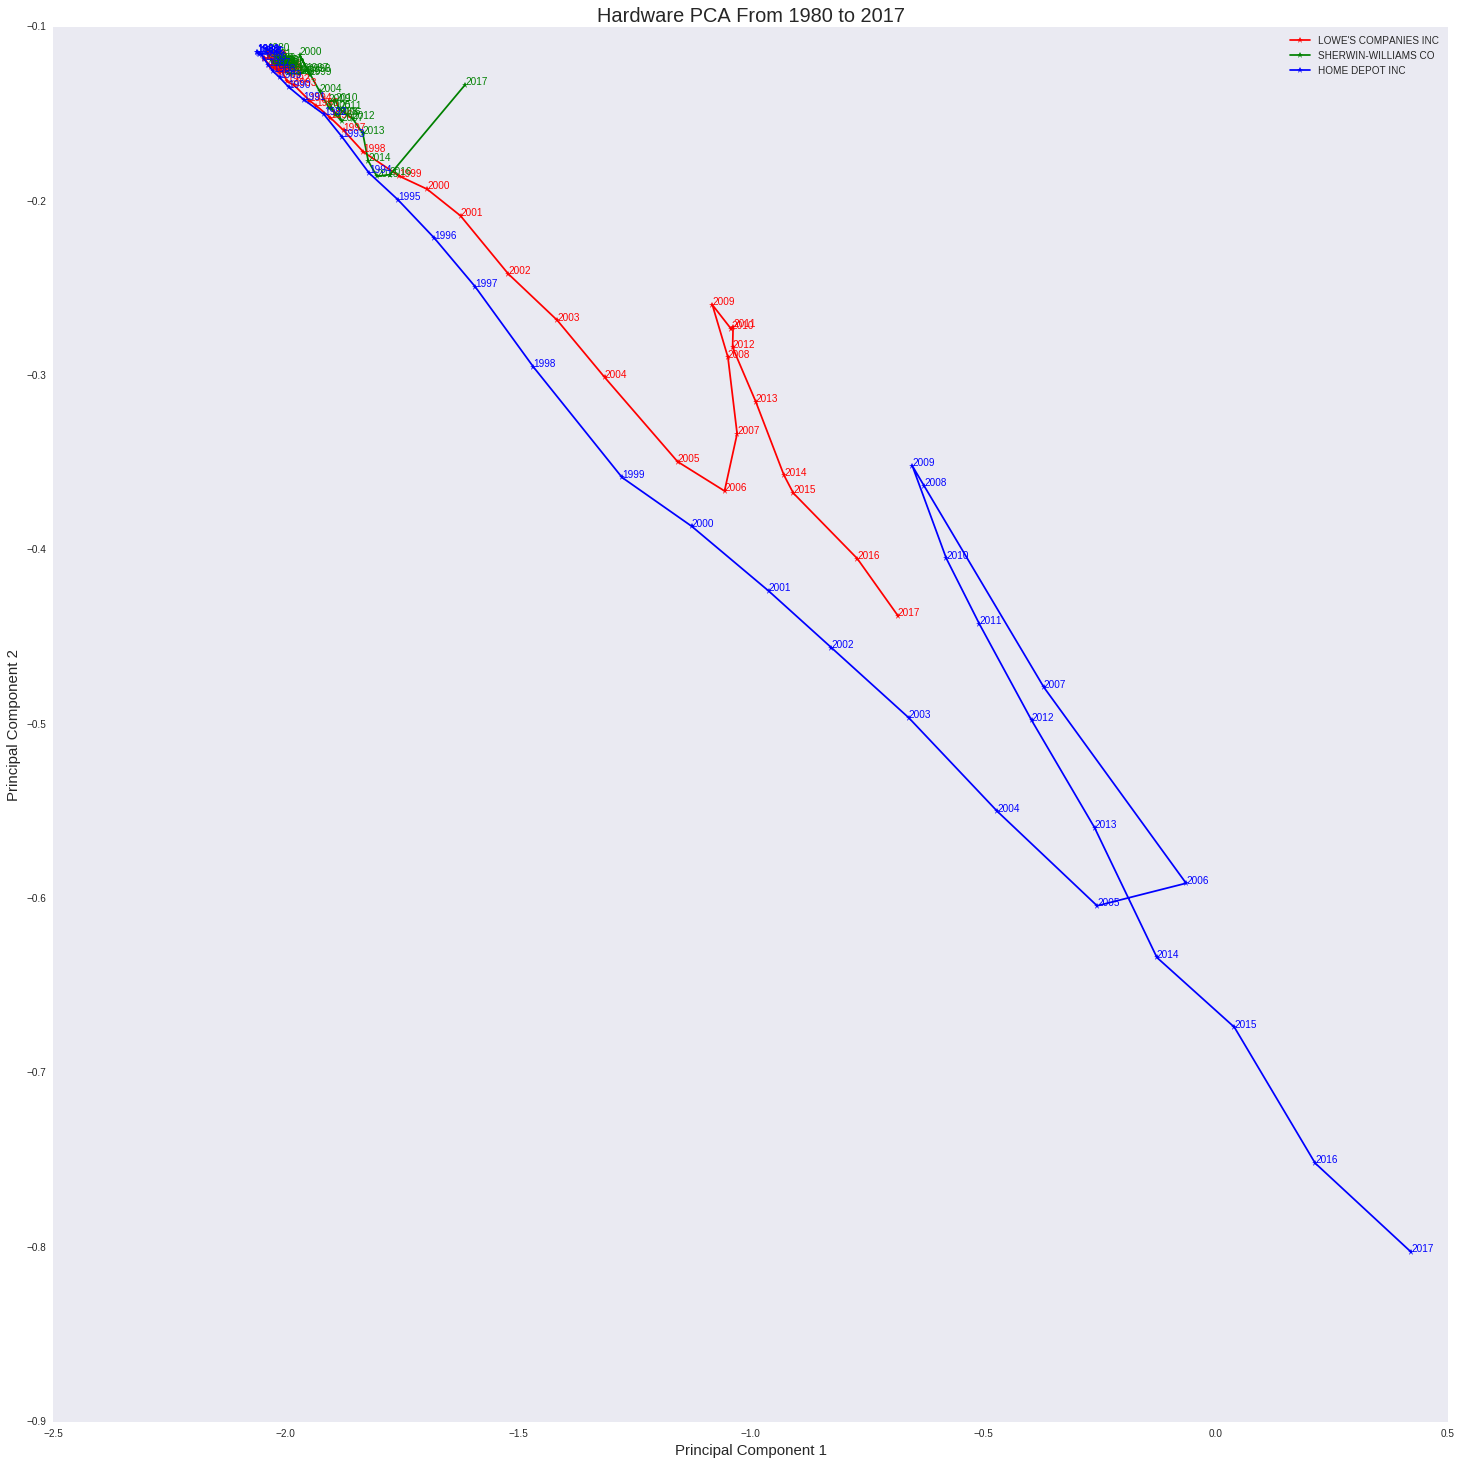
\includegraphics[width=1\textwidth]{./Hardware}\\[0.1in] \\
\subsection{Lowe's Companies Inc}
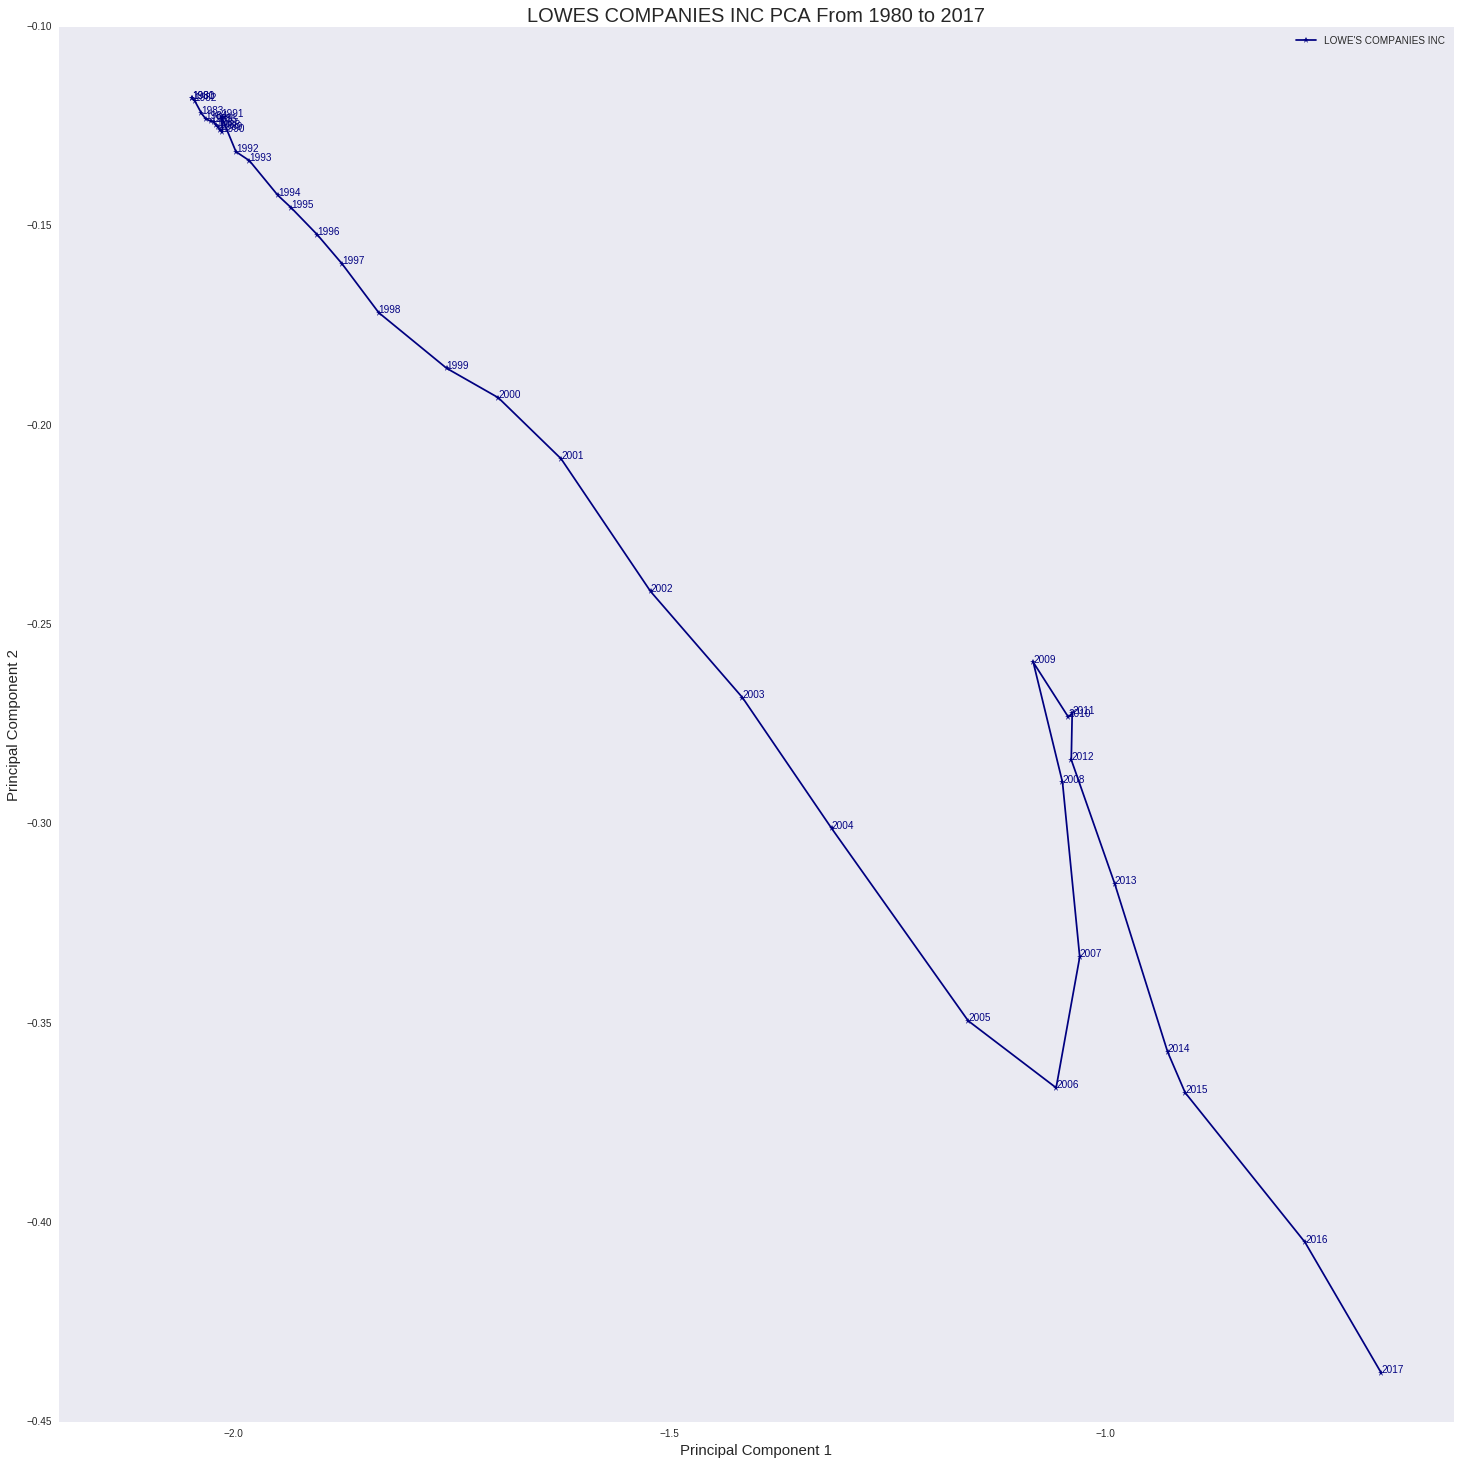
\includegraphics[width=1\textwidth]{./Lowes}\\[0.1in] \\
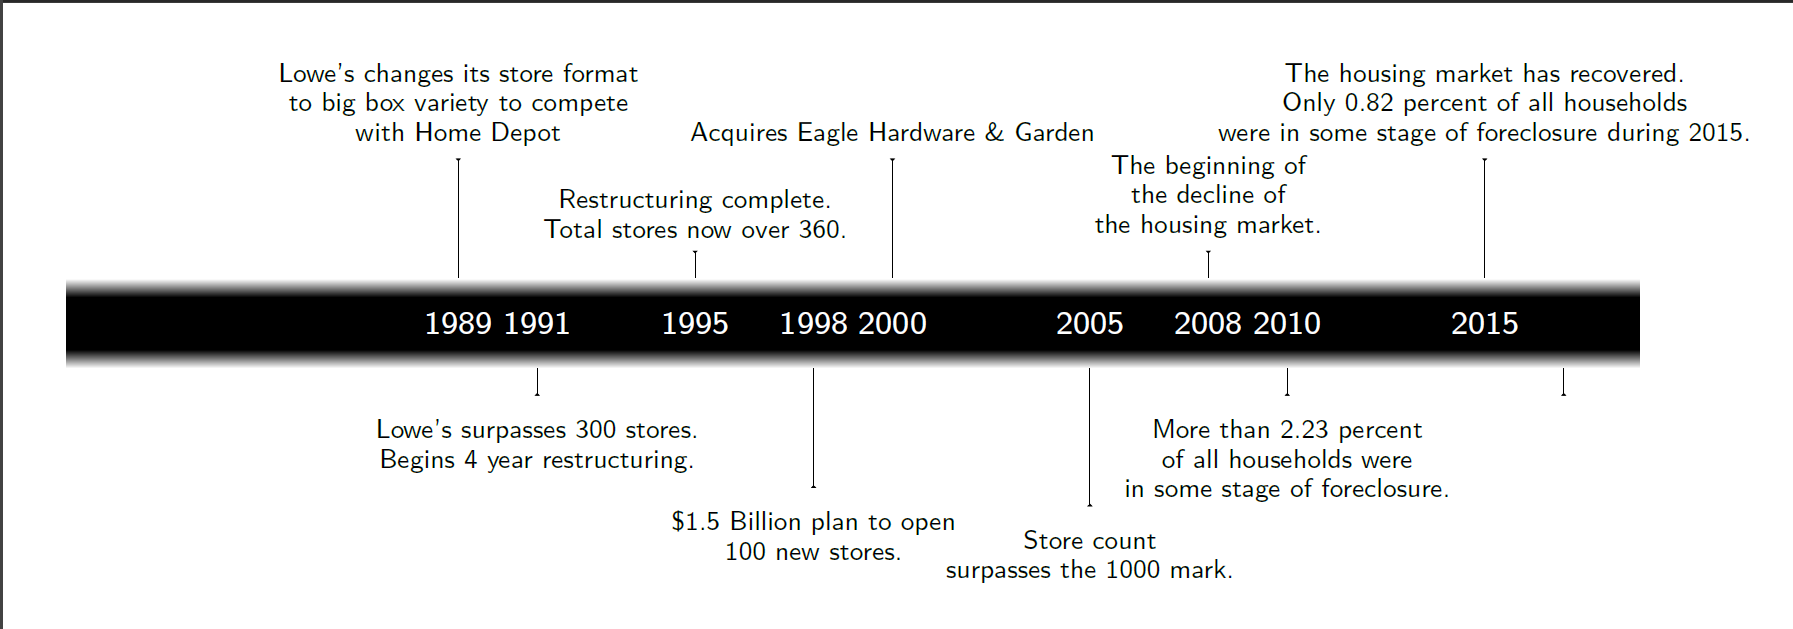
\includegraphics[width=1\textwidth]{./Lowestimeline}\\[0.1in] \\
\subsection{Home Depot Inc}
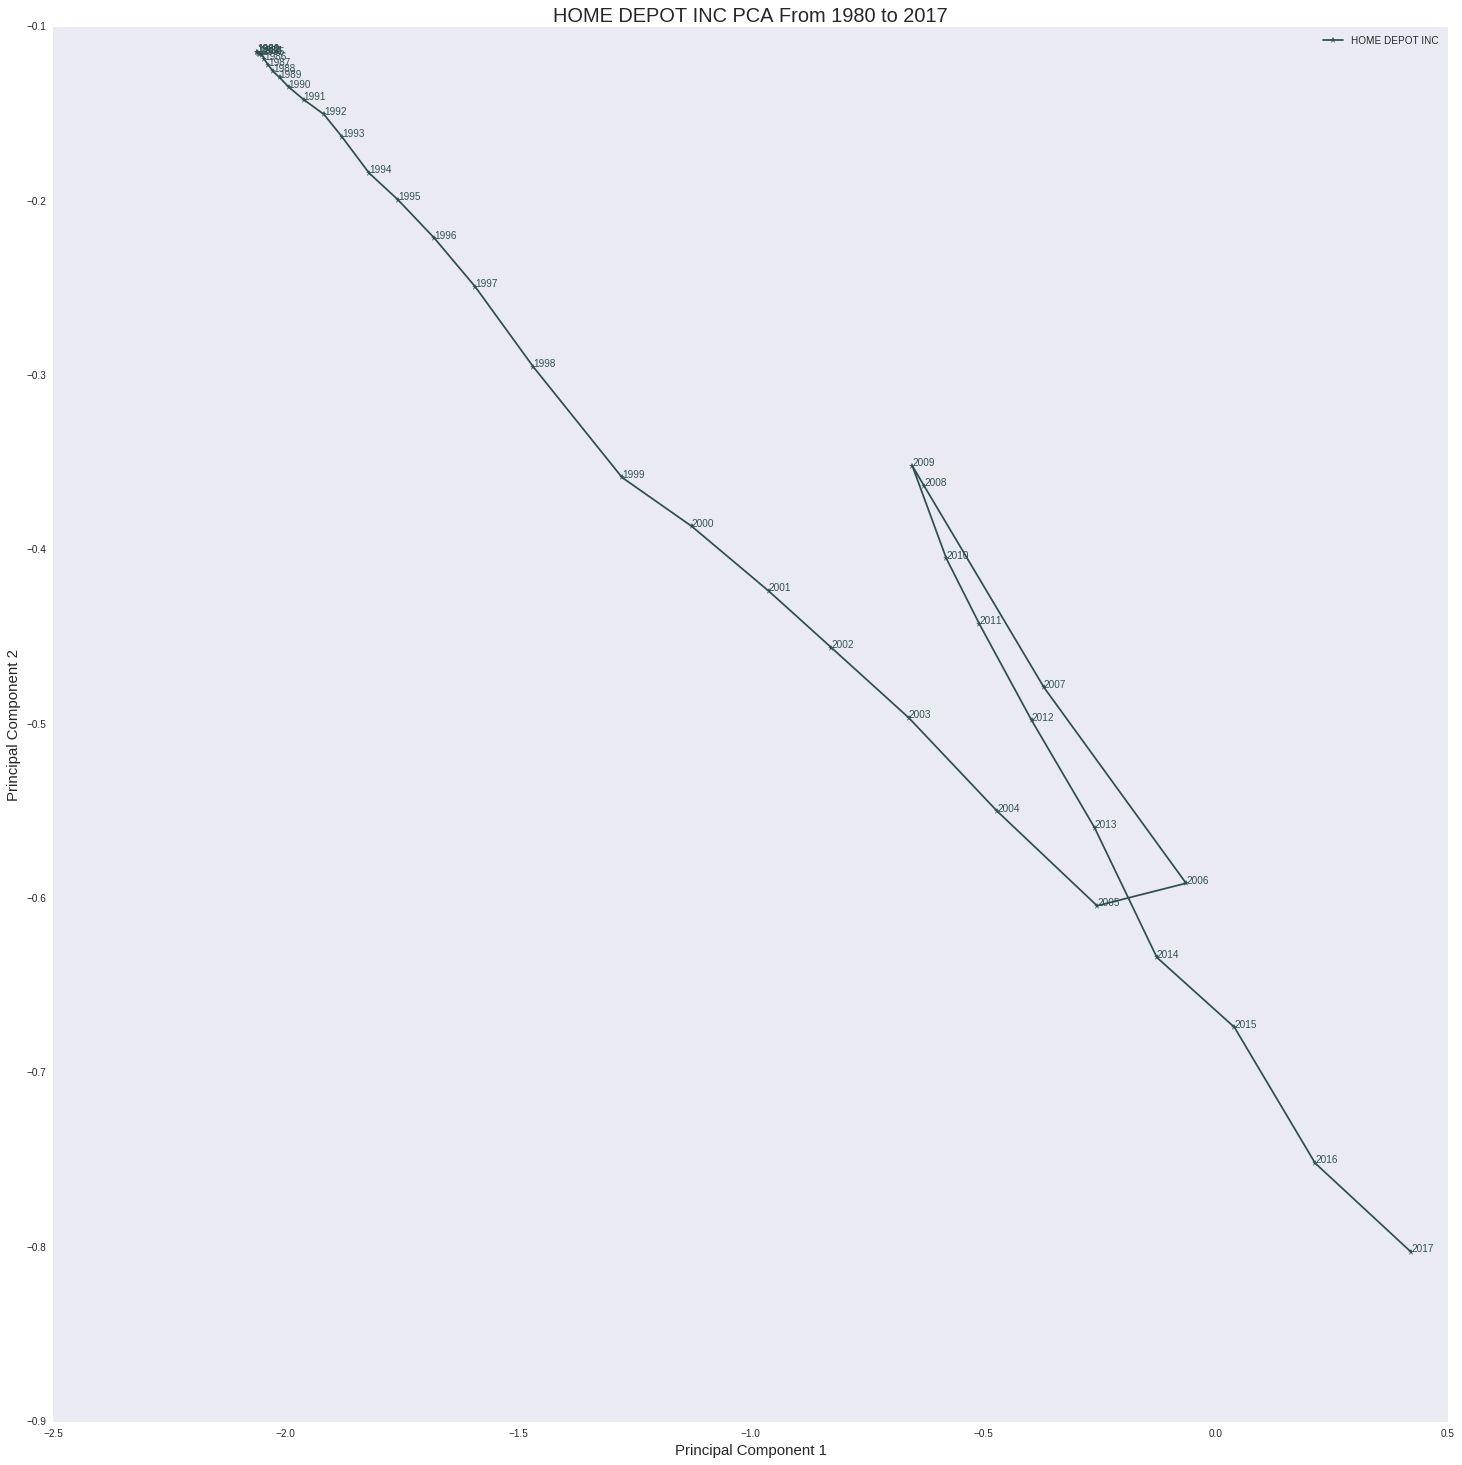
\includegraphics[width=1\textwidth]{./Home_Depot}\\[0.1in] \\
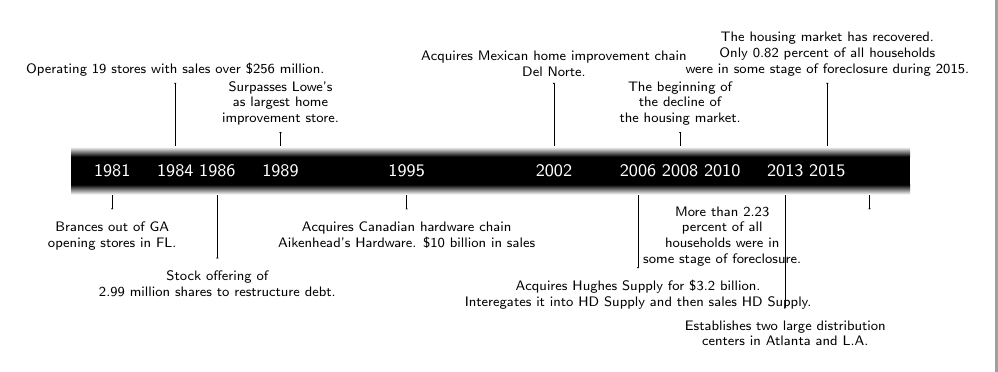
\includegraphics[width=1\textwidth]{./Home_Depottimeline}\\[0.1in] \\
\subsection{Sherwin-Williams Co}
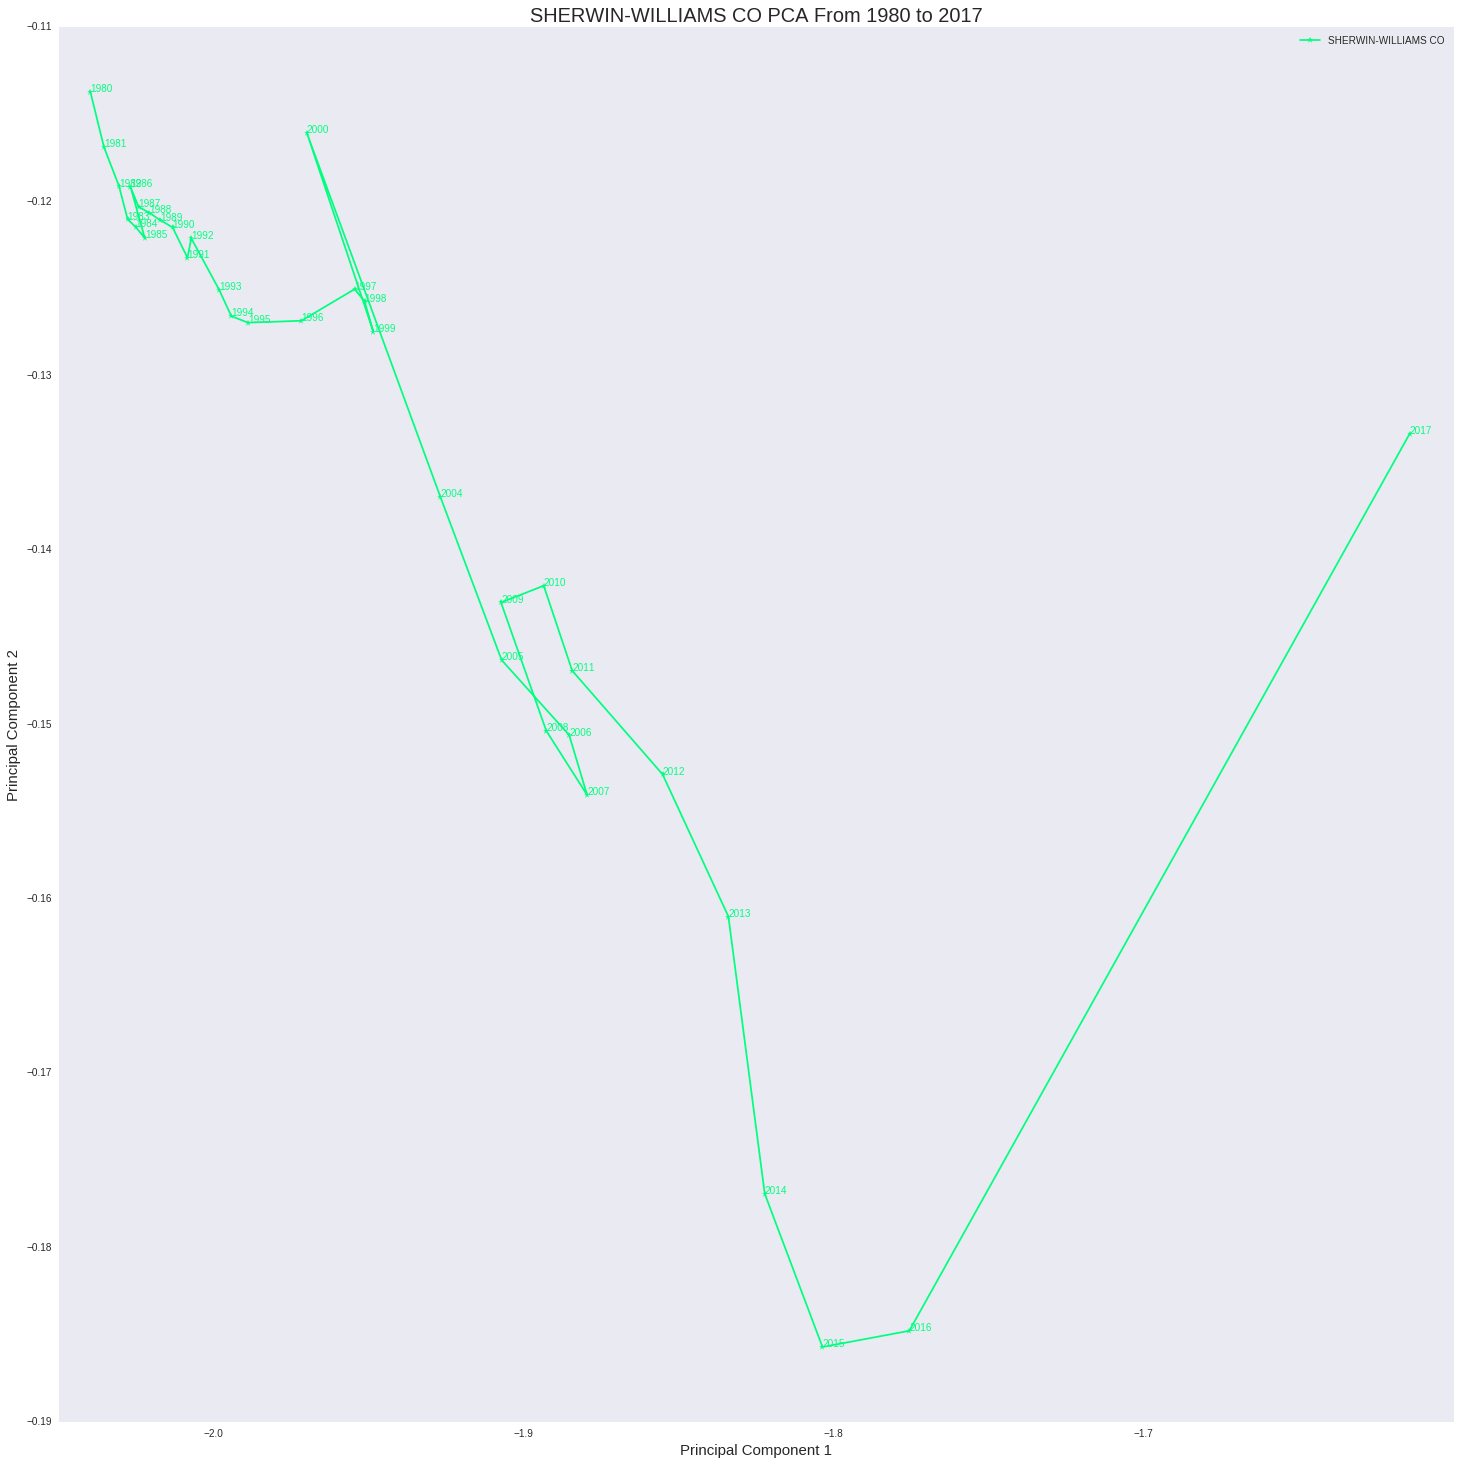
\includegraphics[width=1\textwidth]{./Sherwin_Williams}\\[0.1in] \\
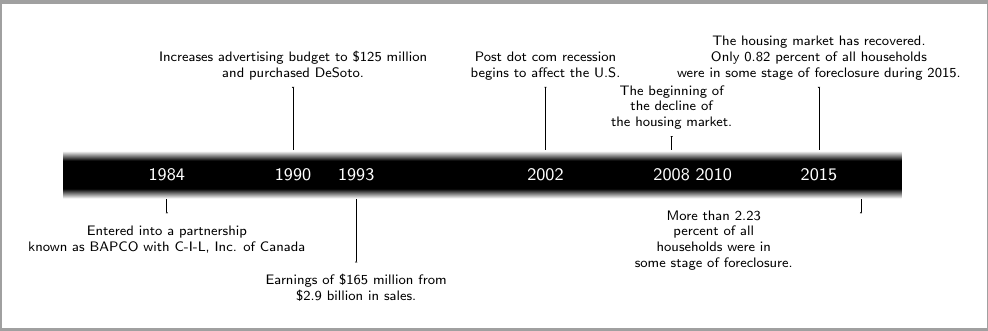
\includegraphics[width=1\textwidth]{./Sherwin_Williamstimeline}\\[0.1in] \\

\section{Retail}
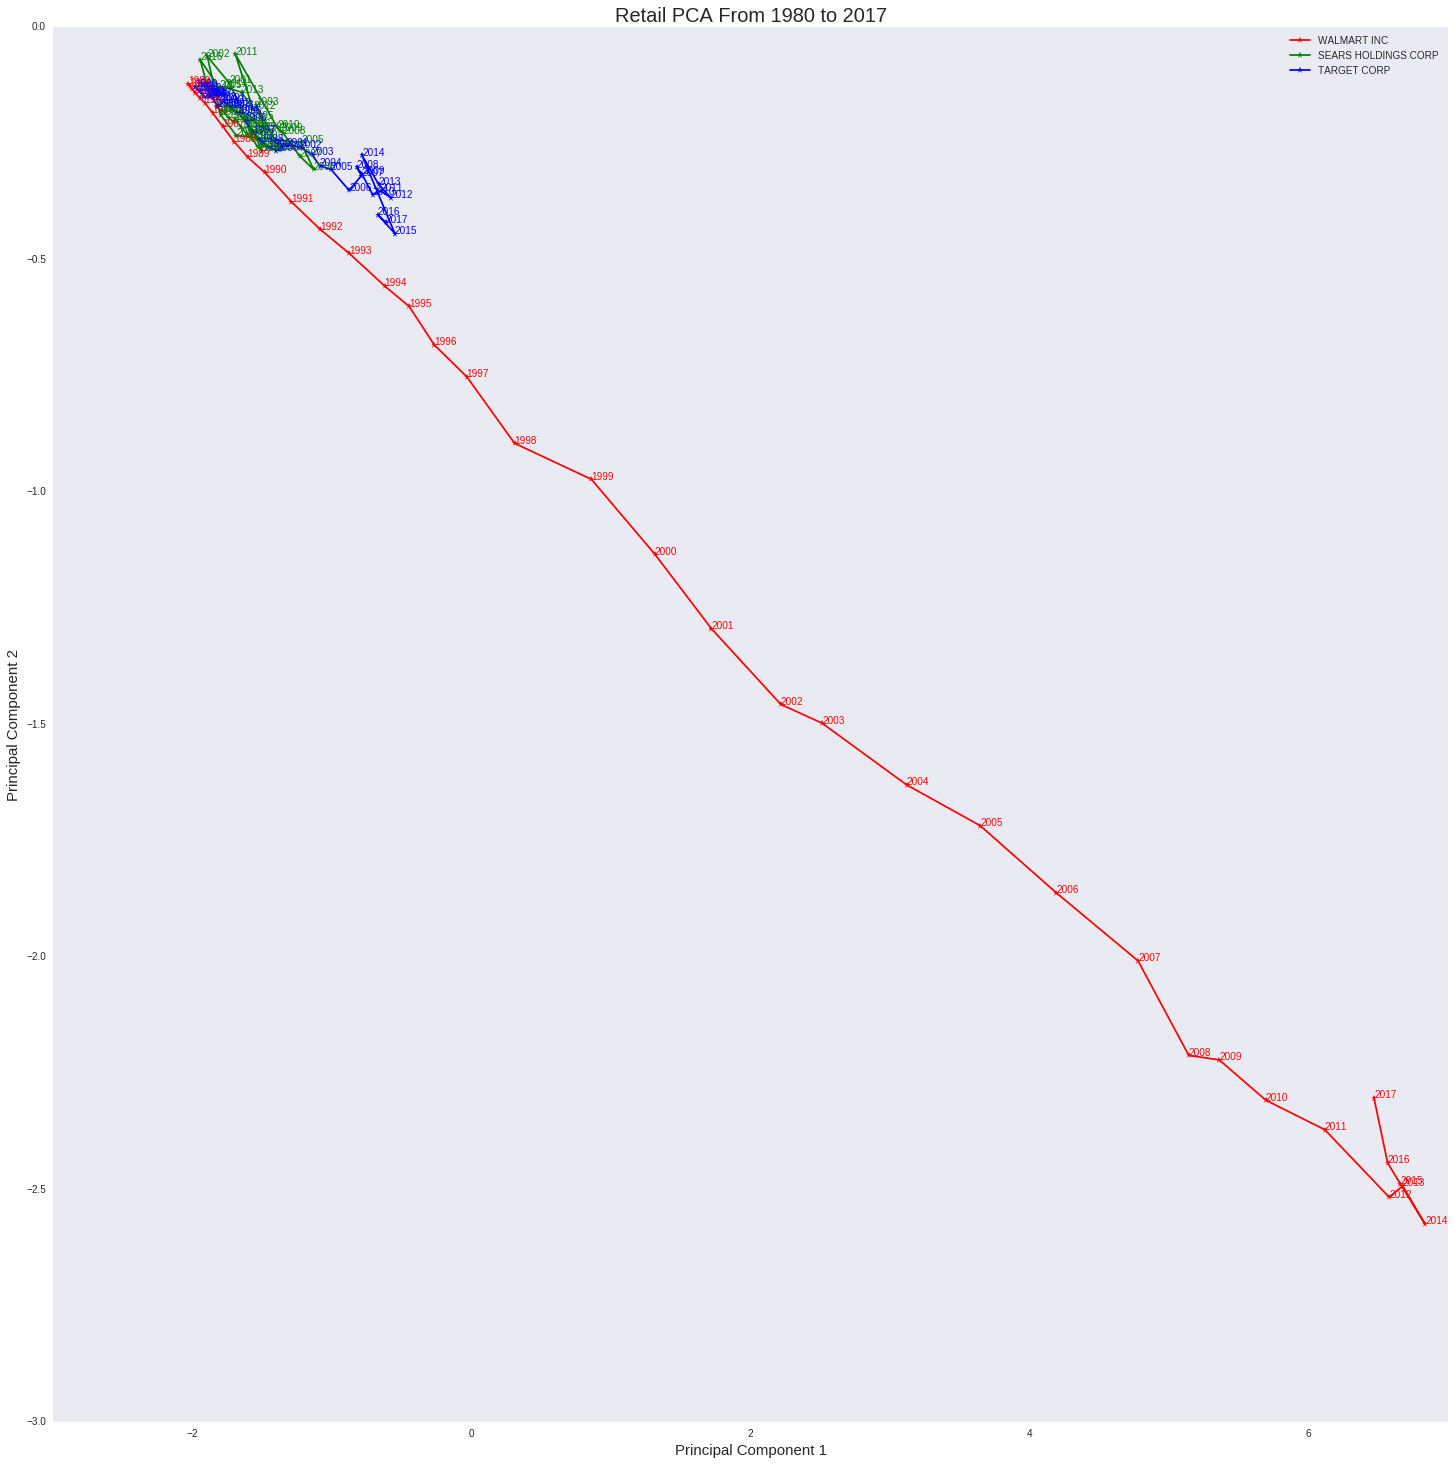
\includegraphics[width=1\textwidth]{./Retail}\\[0.1in] \\
\subsection{WalMart Inc}
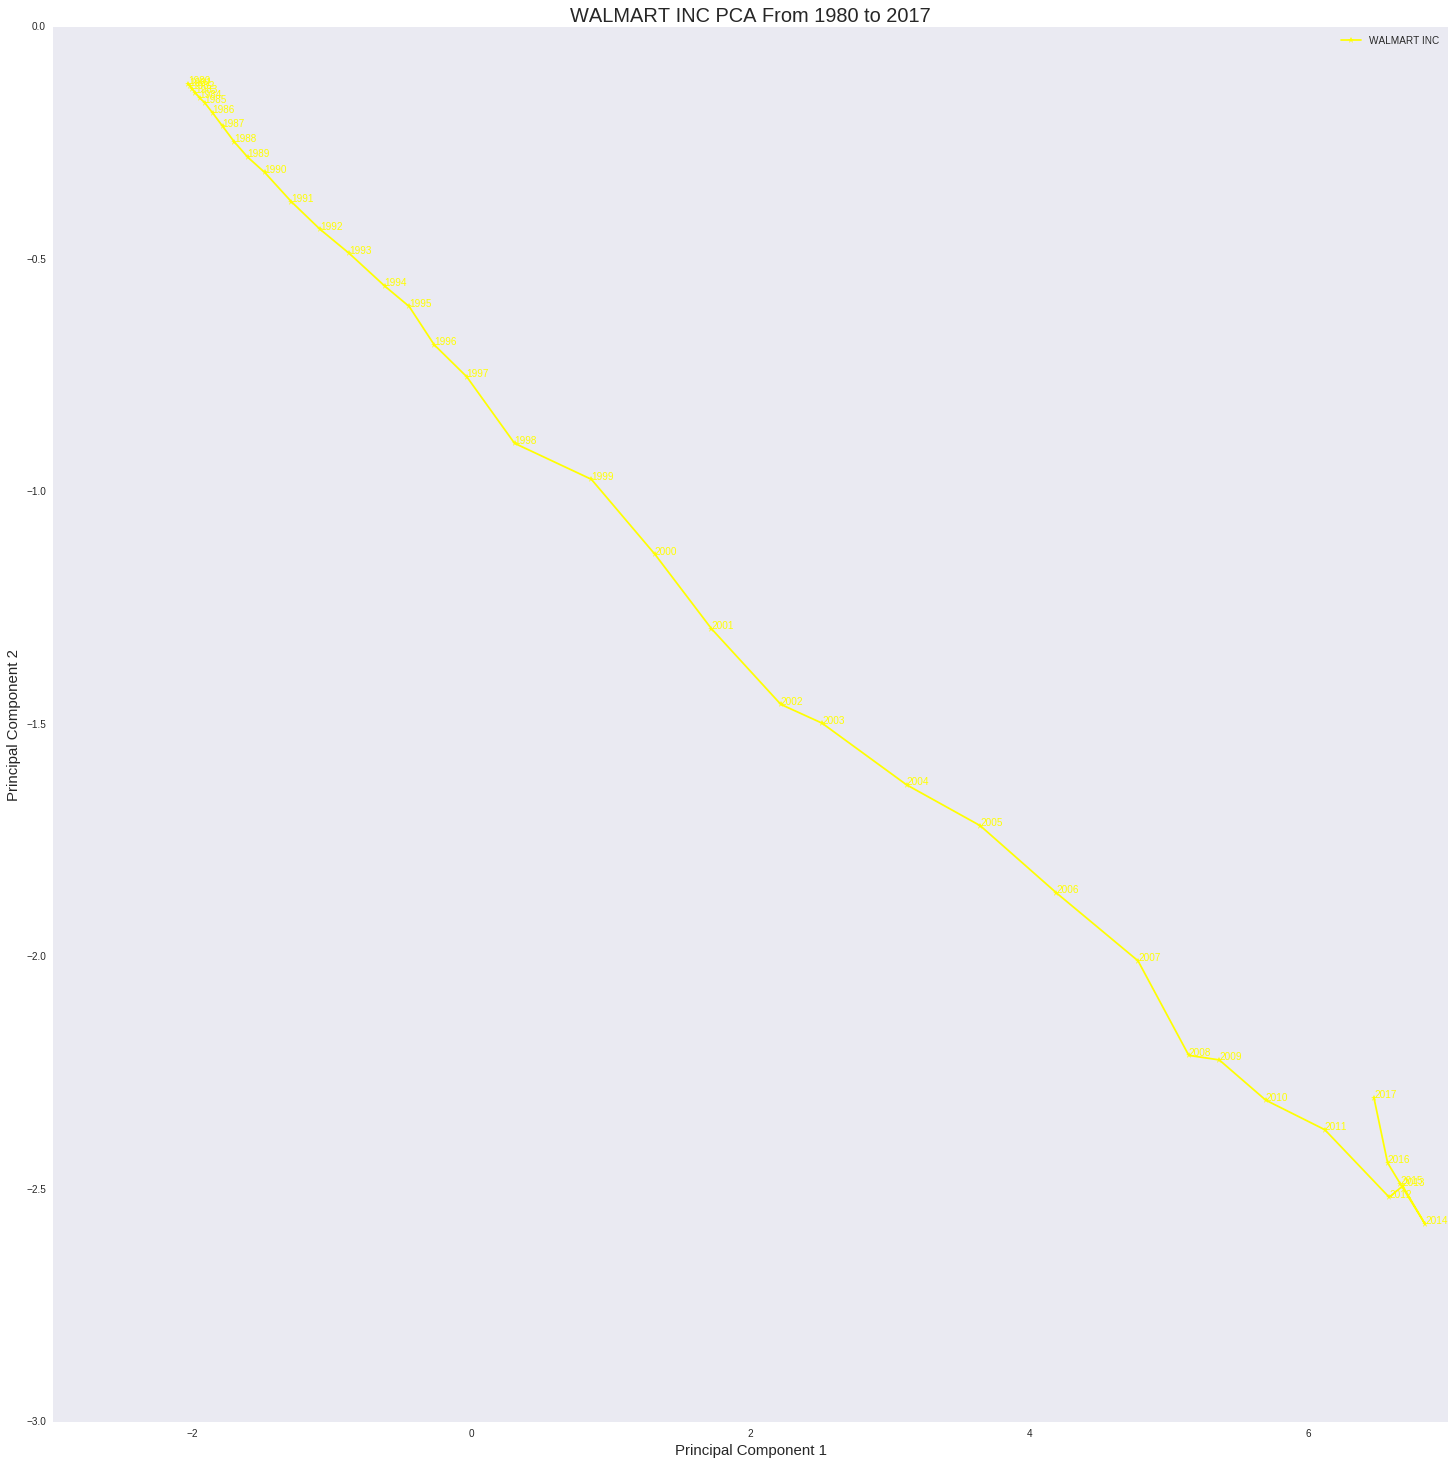
\includegraphics[width=1\textwidth]{./WalMart}\\[0.1in] \\
\subsection{Sears Holdings Corp}
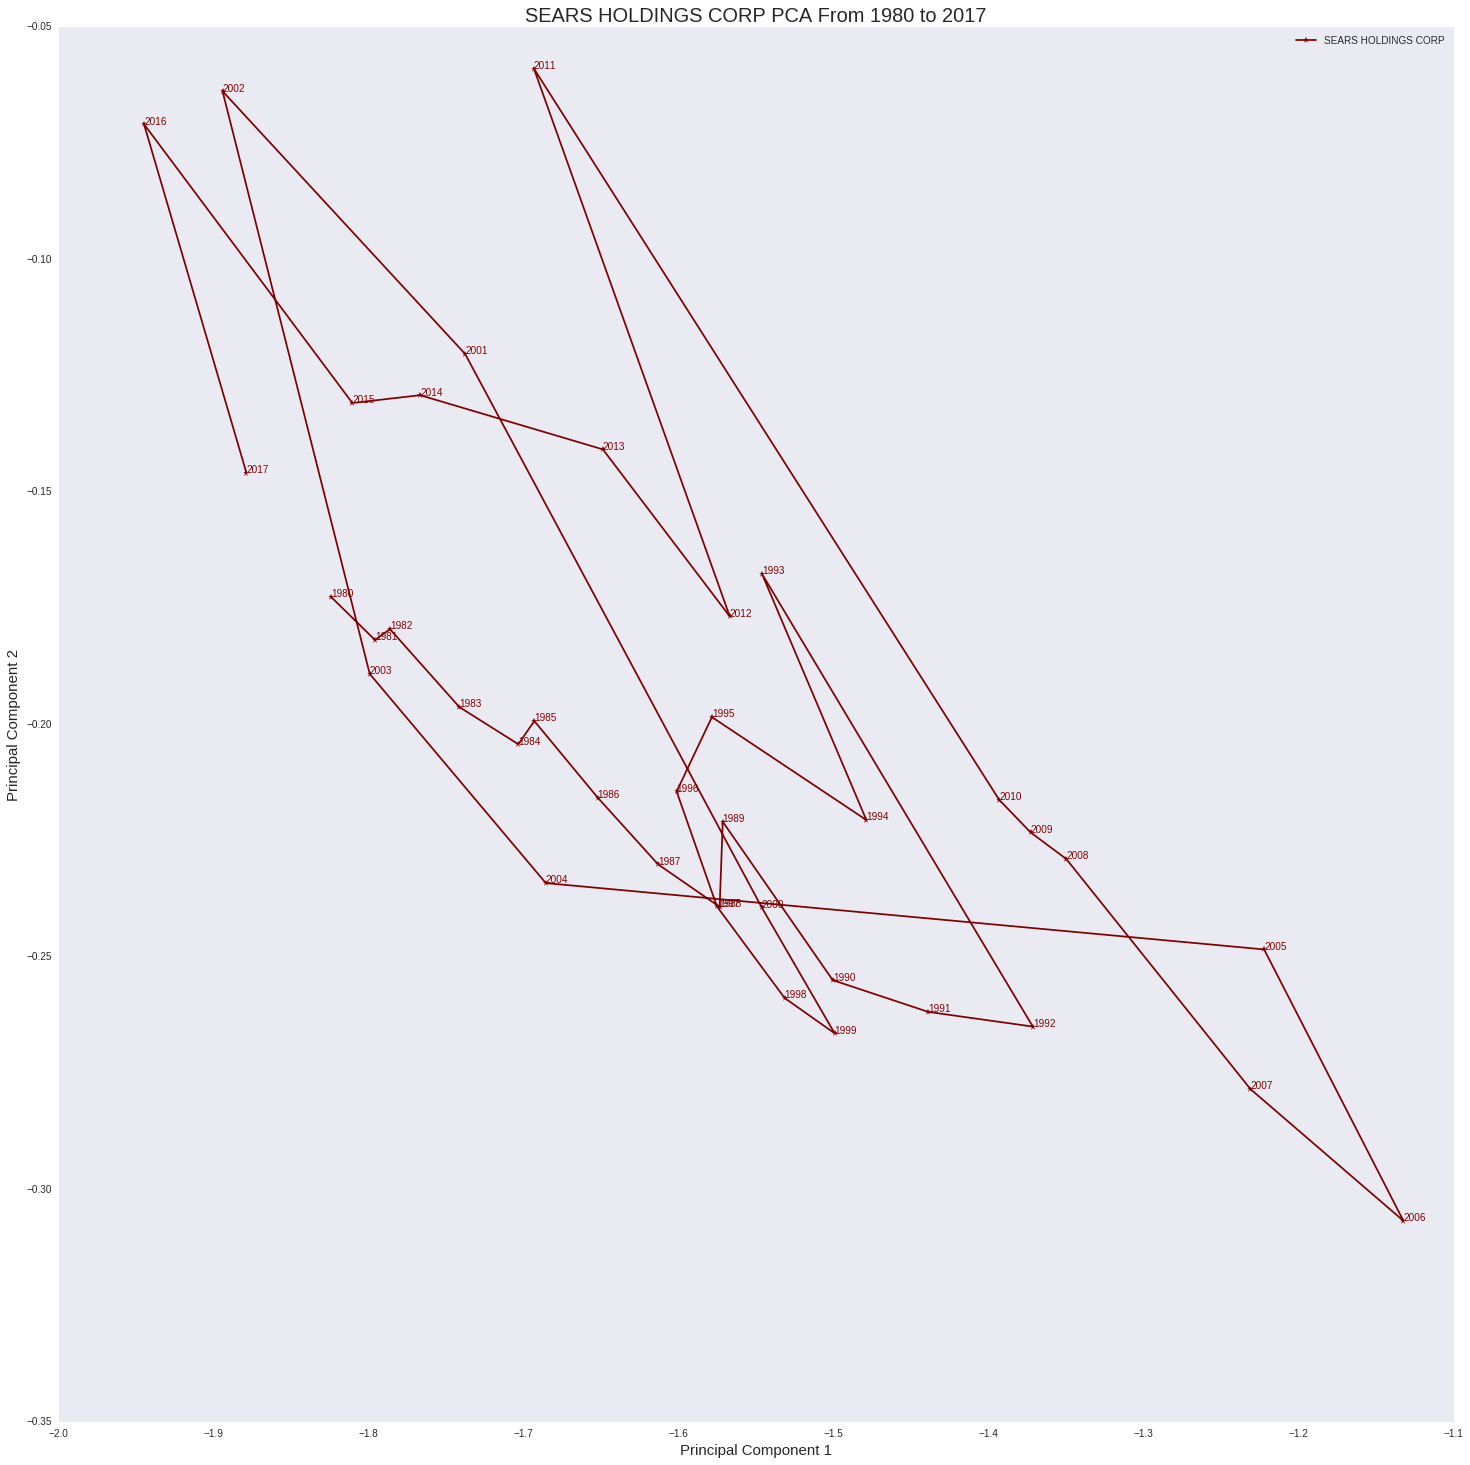
\includegraphics[width=1\textwidth]{./Sears}\\[0.1in] \\
\subsection{Target Corp}
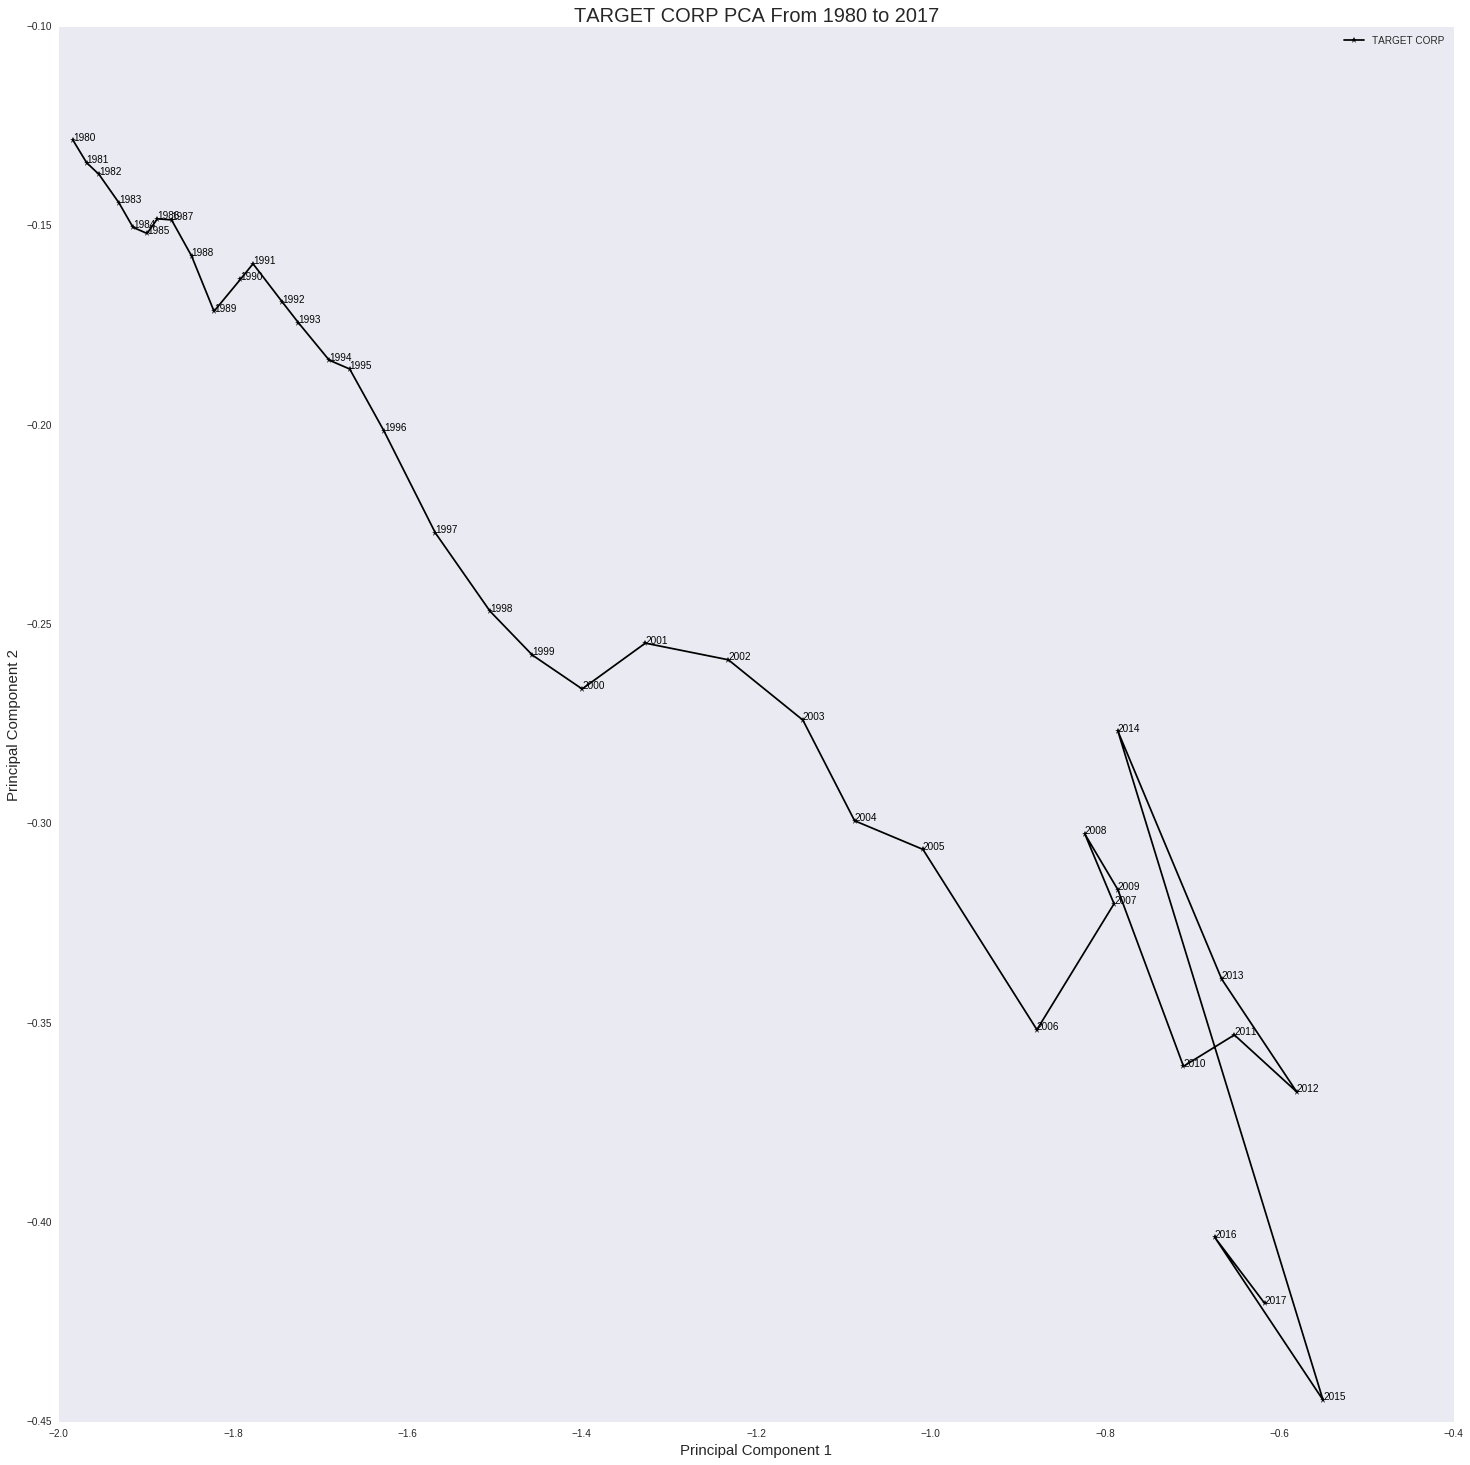
\includegraphics[width=1\textwidth]{./Target}\\[0.1in] \\

\section{Oil}
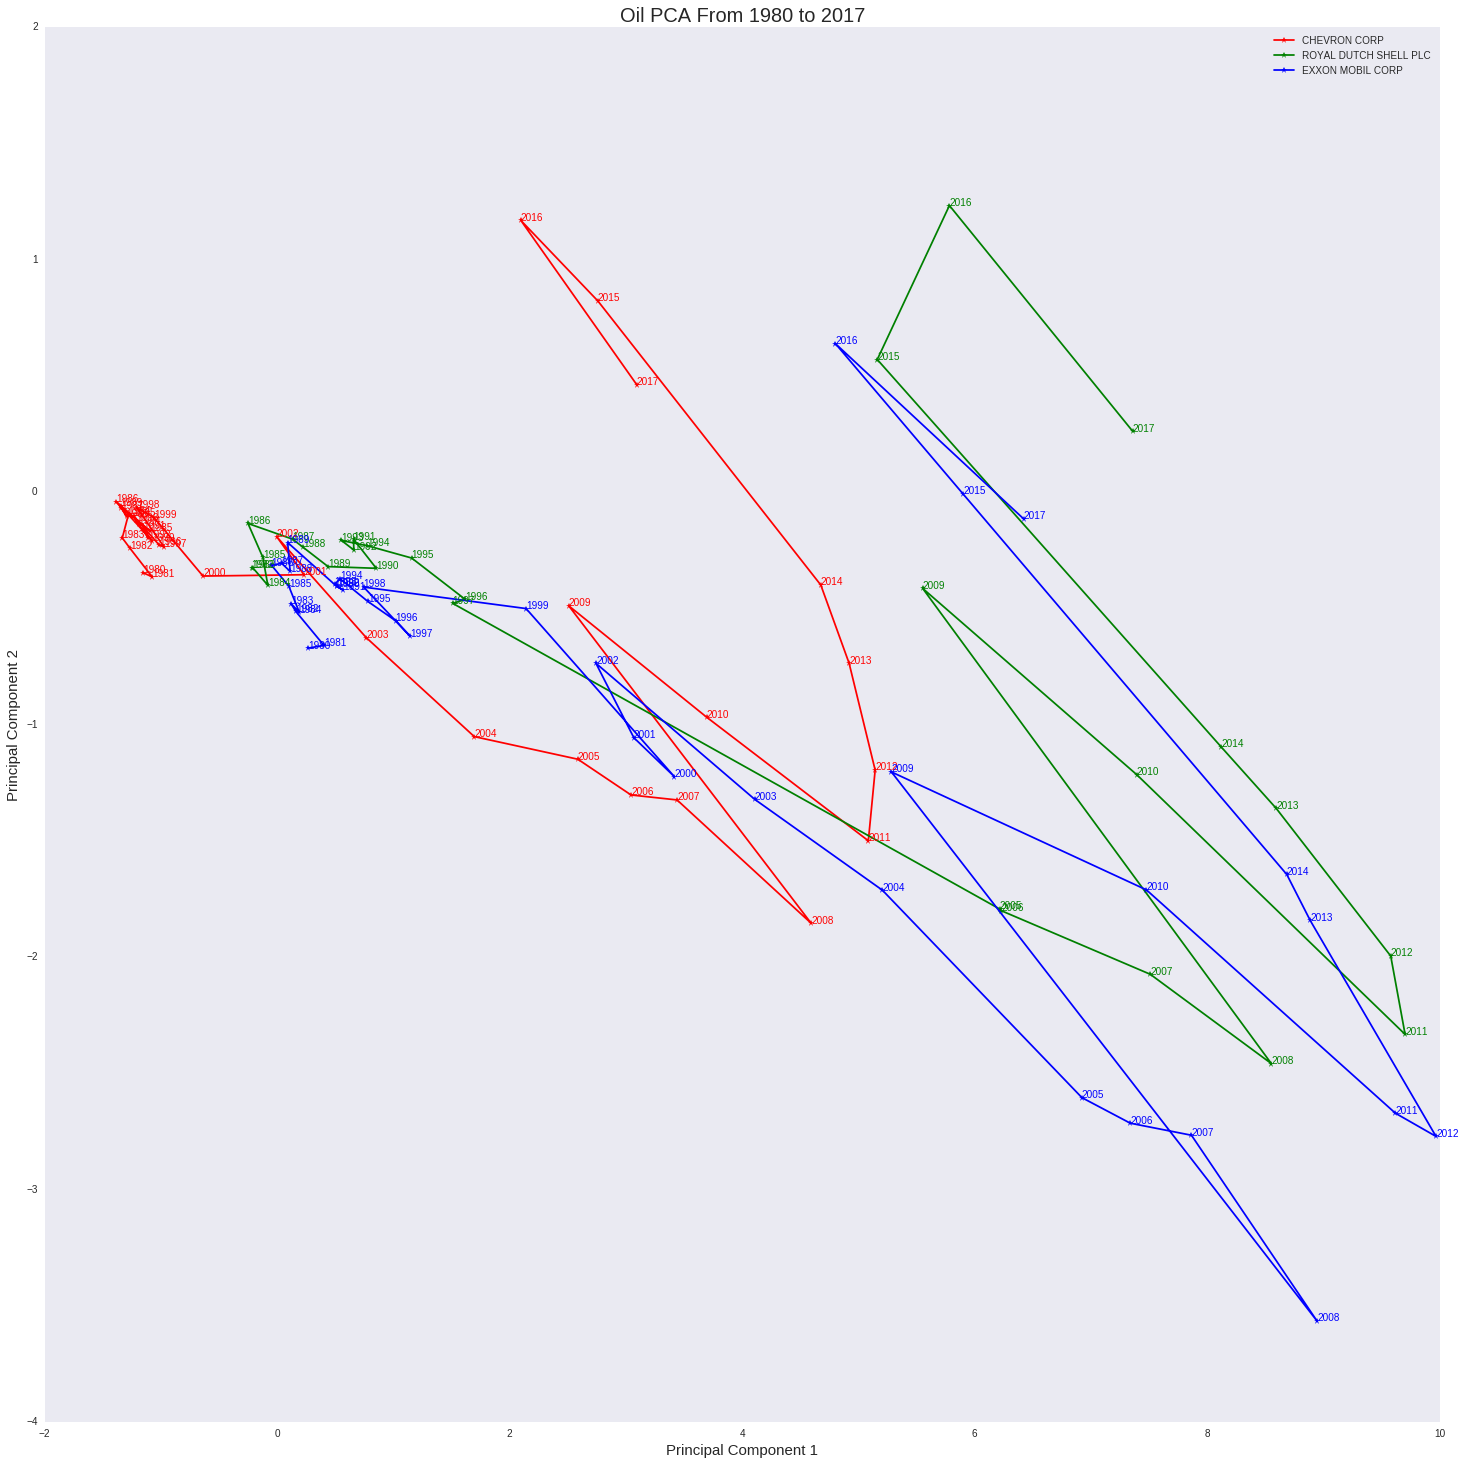
\includegraphics[width=1\textwidth]{./Oil}\\[0.1in] \\
\subsection{Exxon Mobil Corp}
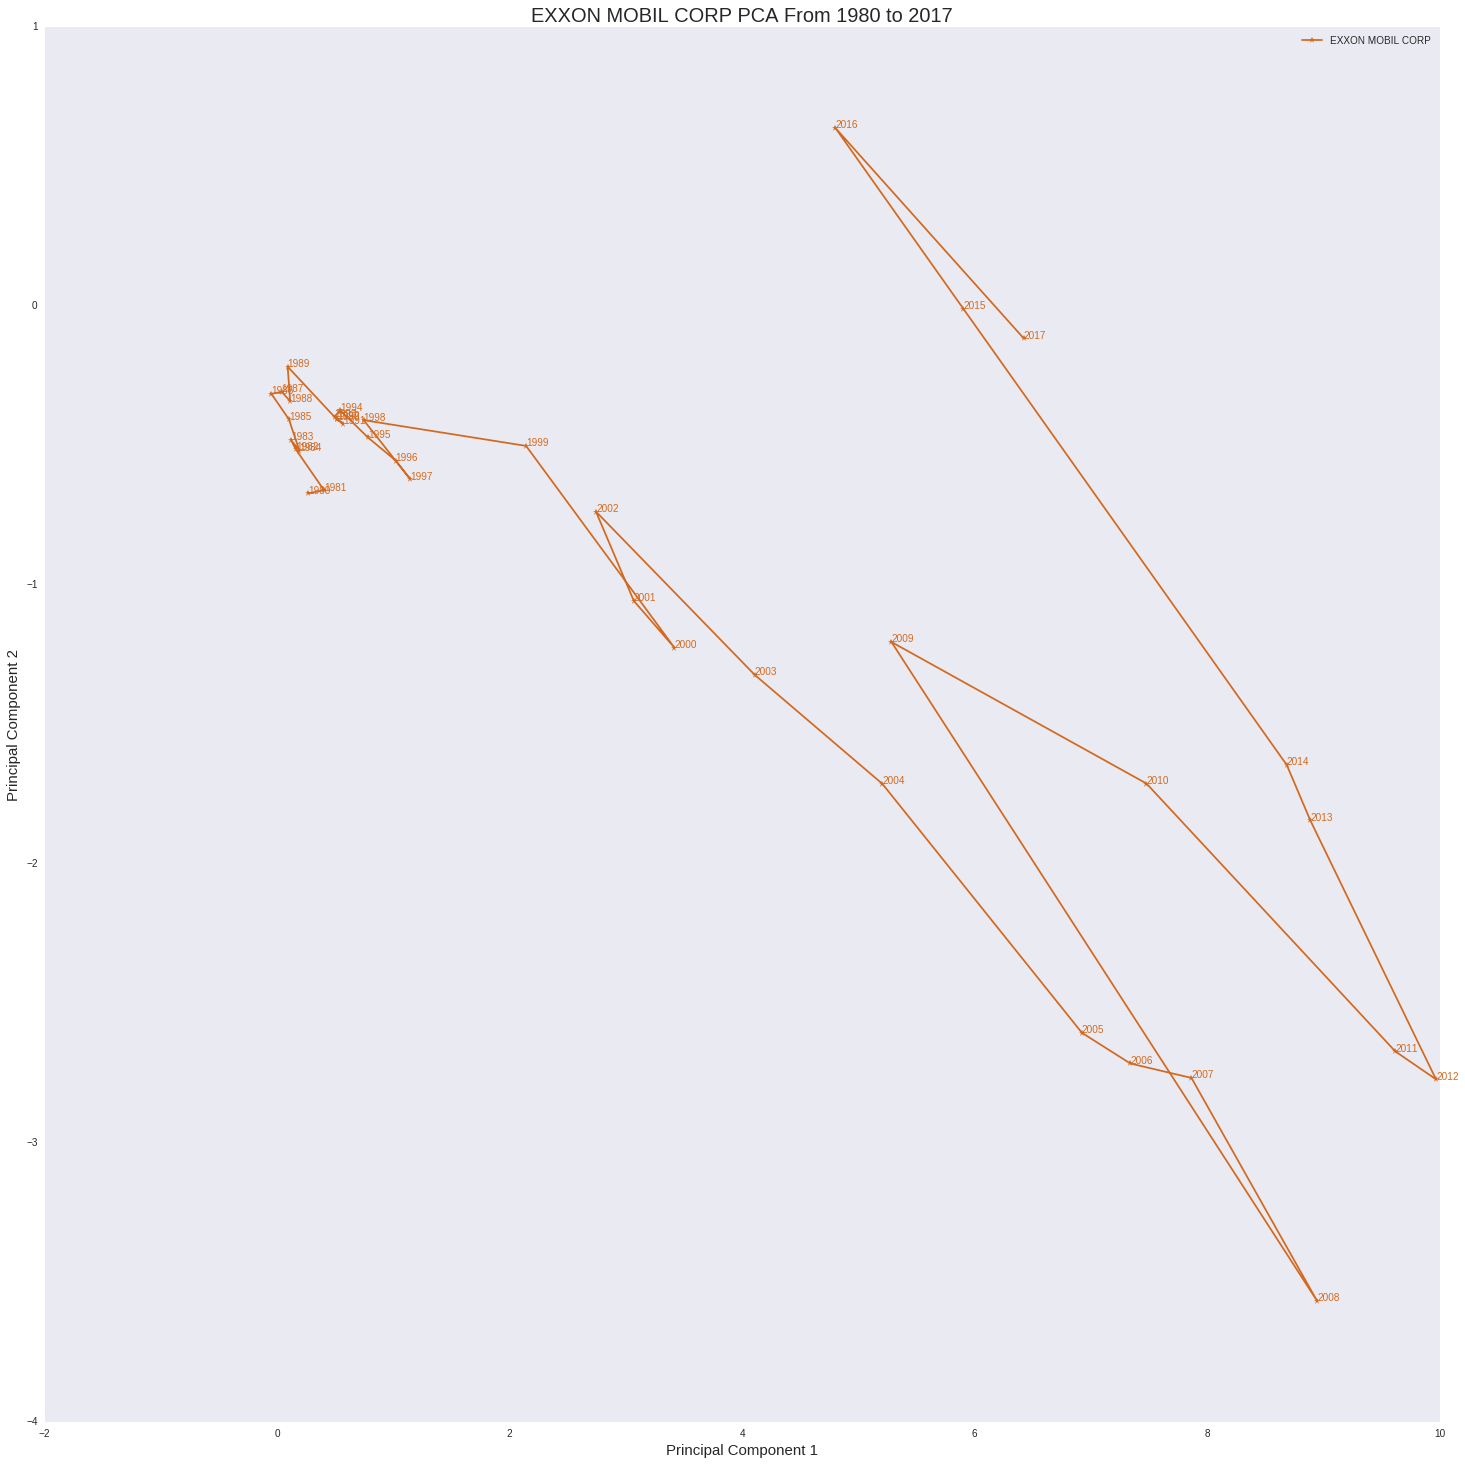
\includegraphics[width=1\textwidth]{./Exxon}\\[0.1in] \\
\subsection{Royal Dutch Shell PLC}
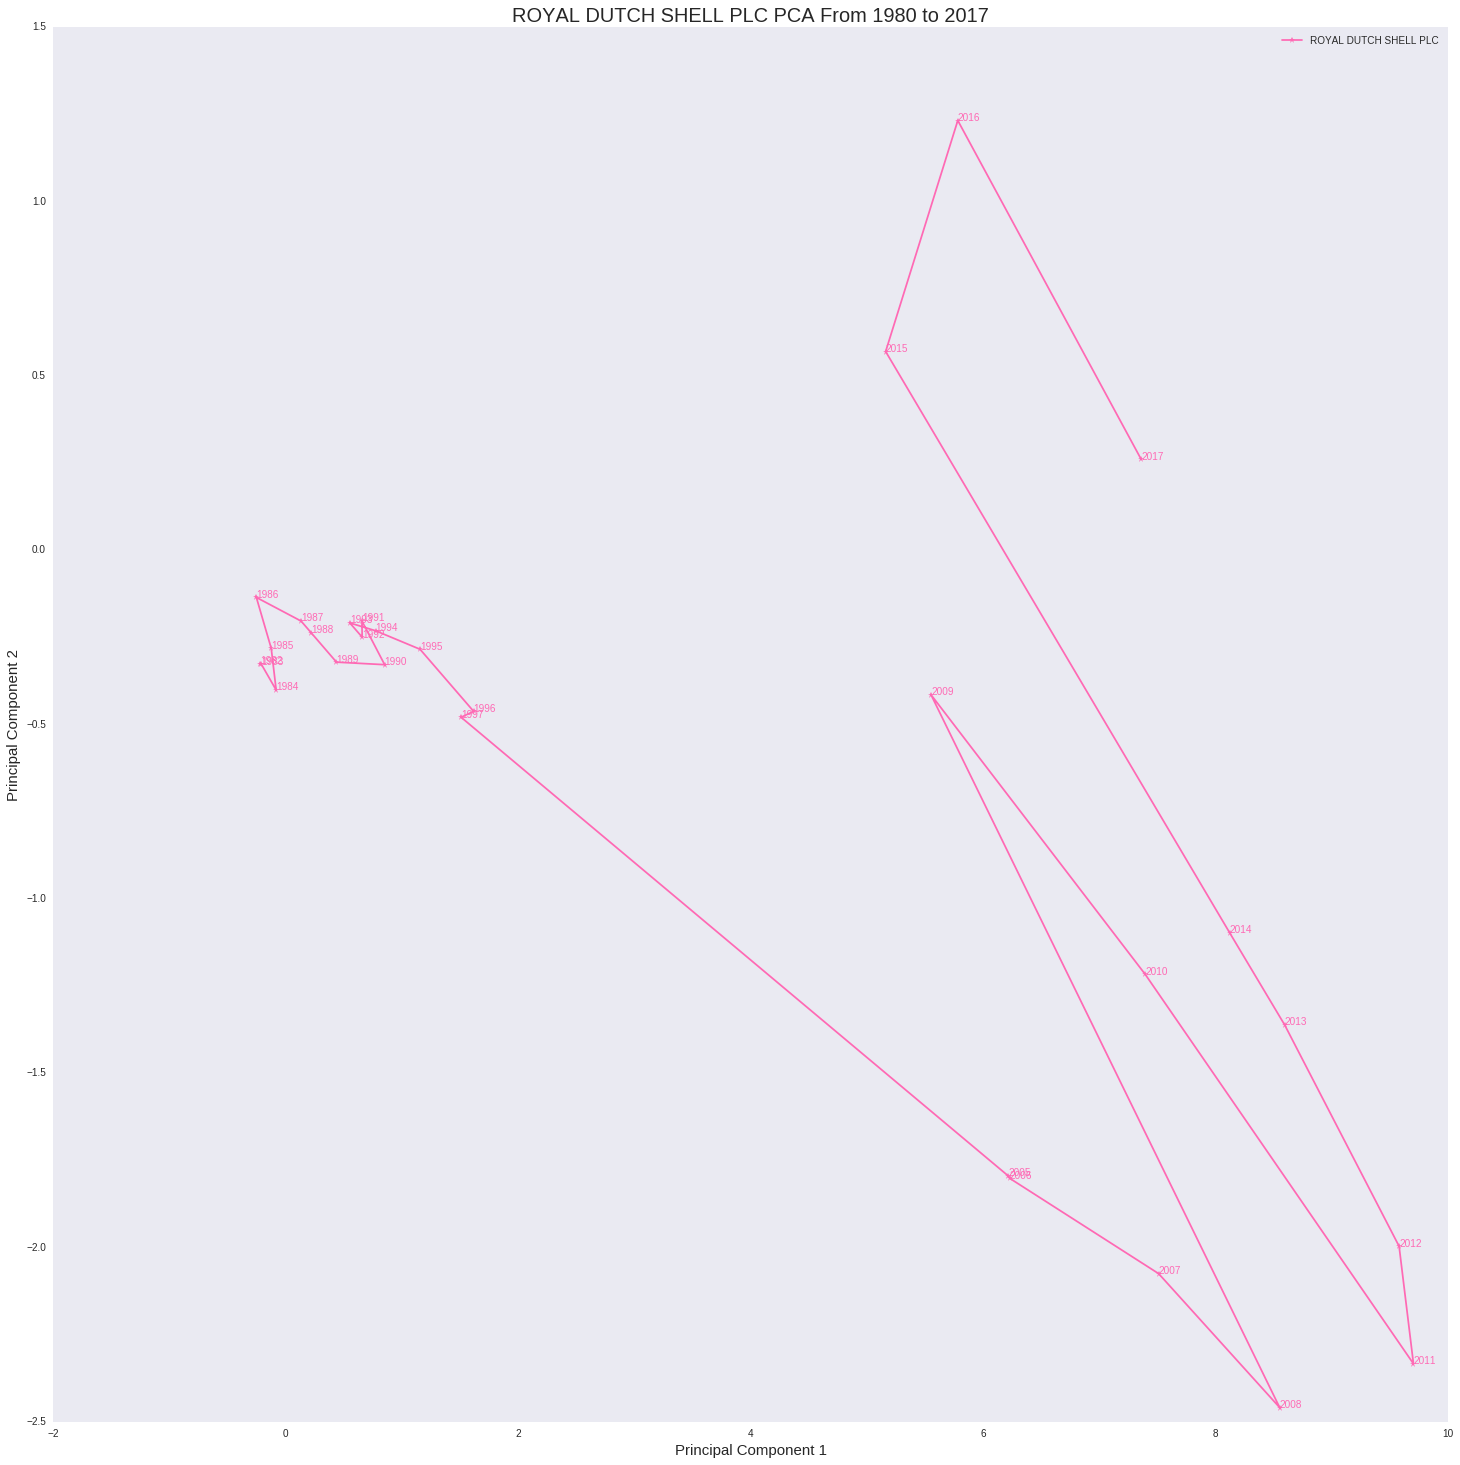
\includegraphics[width=1\textwidth]{./Shell}\\[0.1in] \\
\subsection{Chevron Corp}
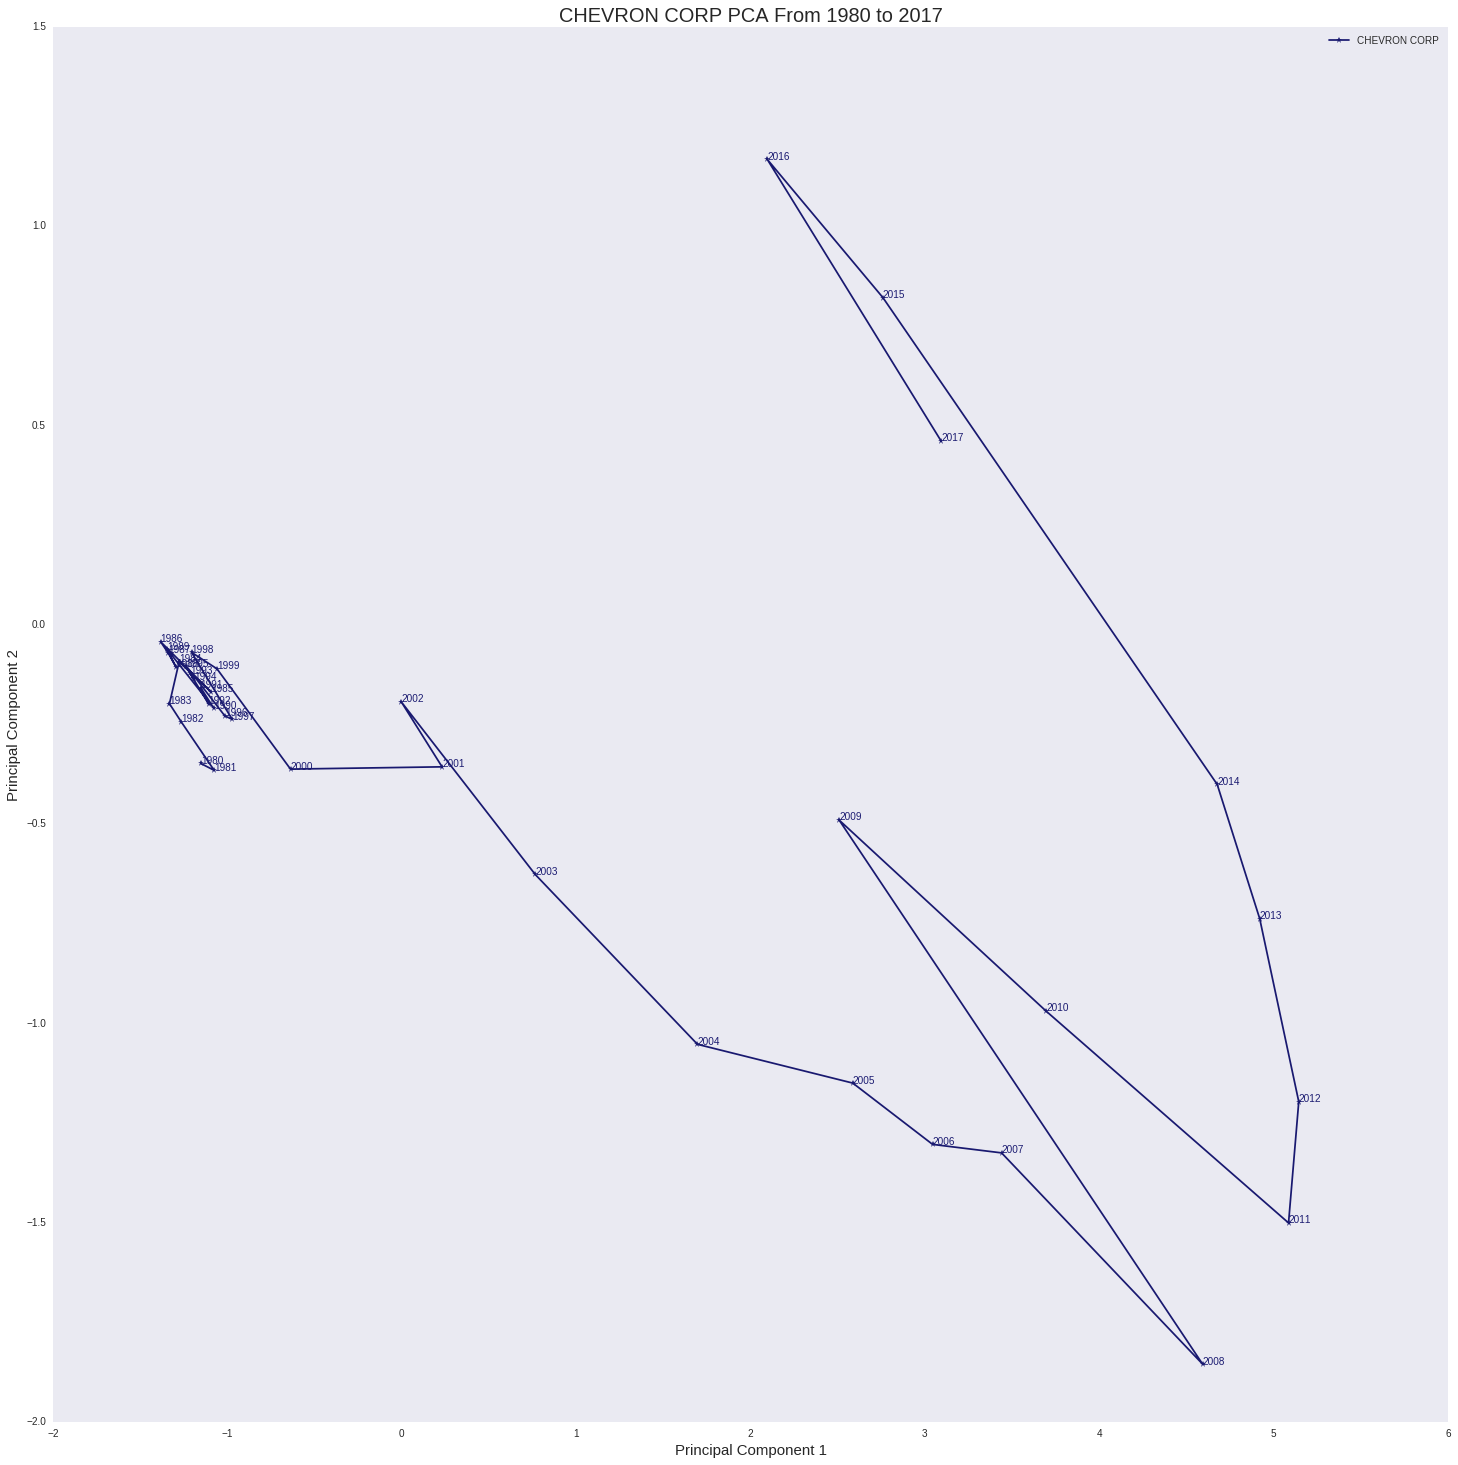
\includegraphics[width=1\textwidth]{./Chevron}\\[0.1in] \\

\section{Automotive}
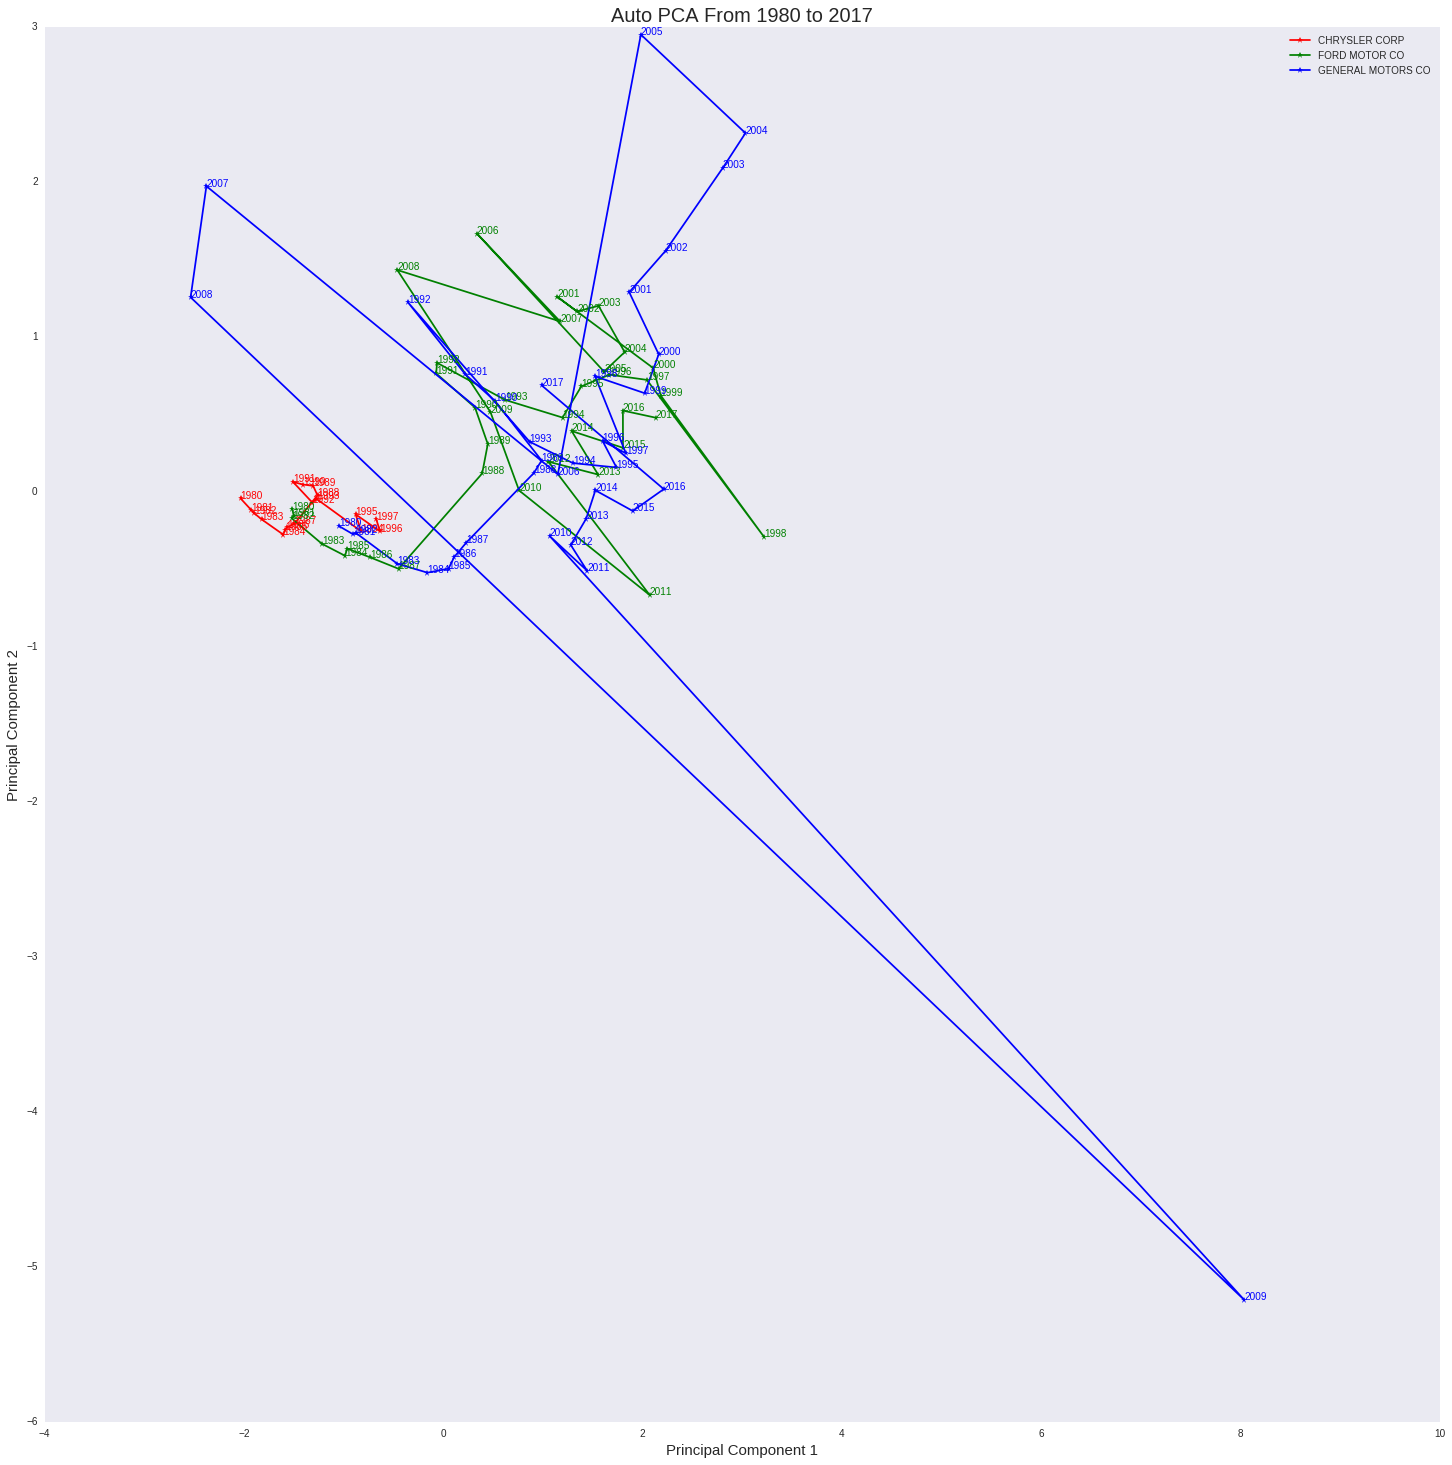
\includegraphics[width=1\textwidth]{./Auto}\\[0.1in] \\
\subsection{Chrysler Corp}
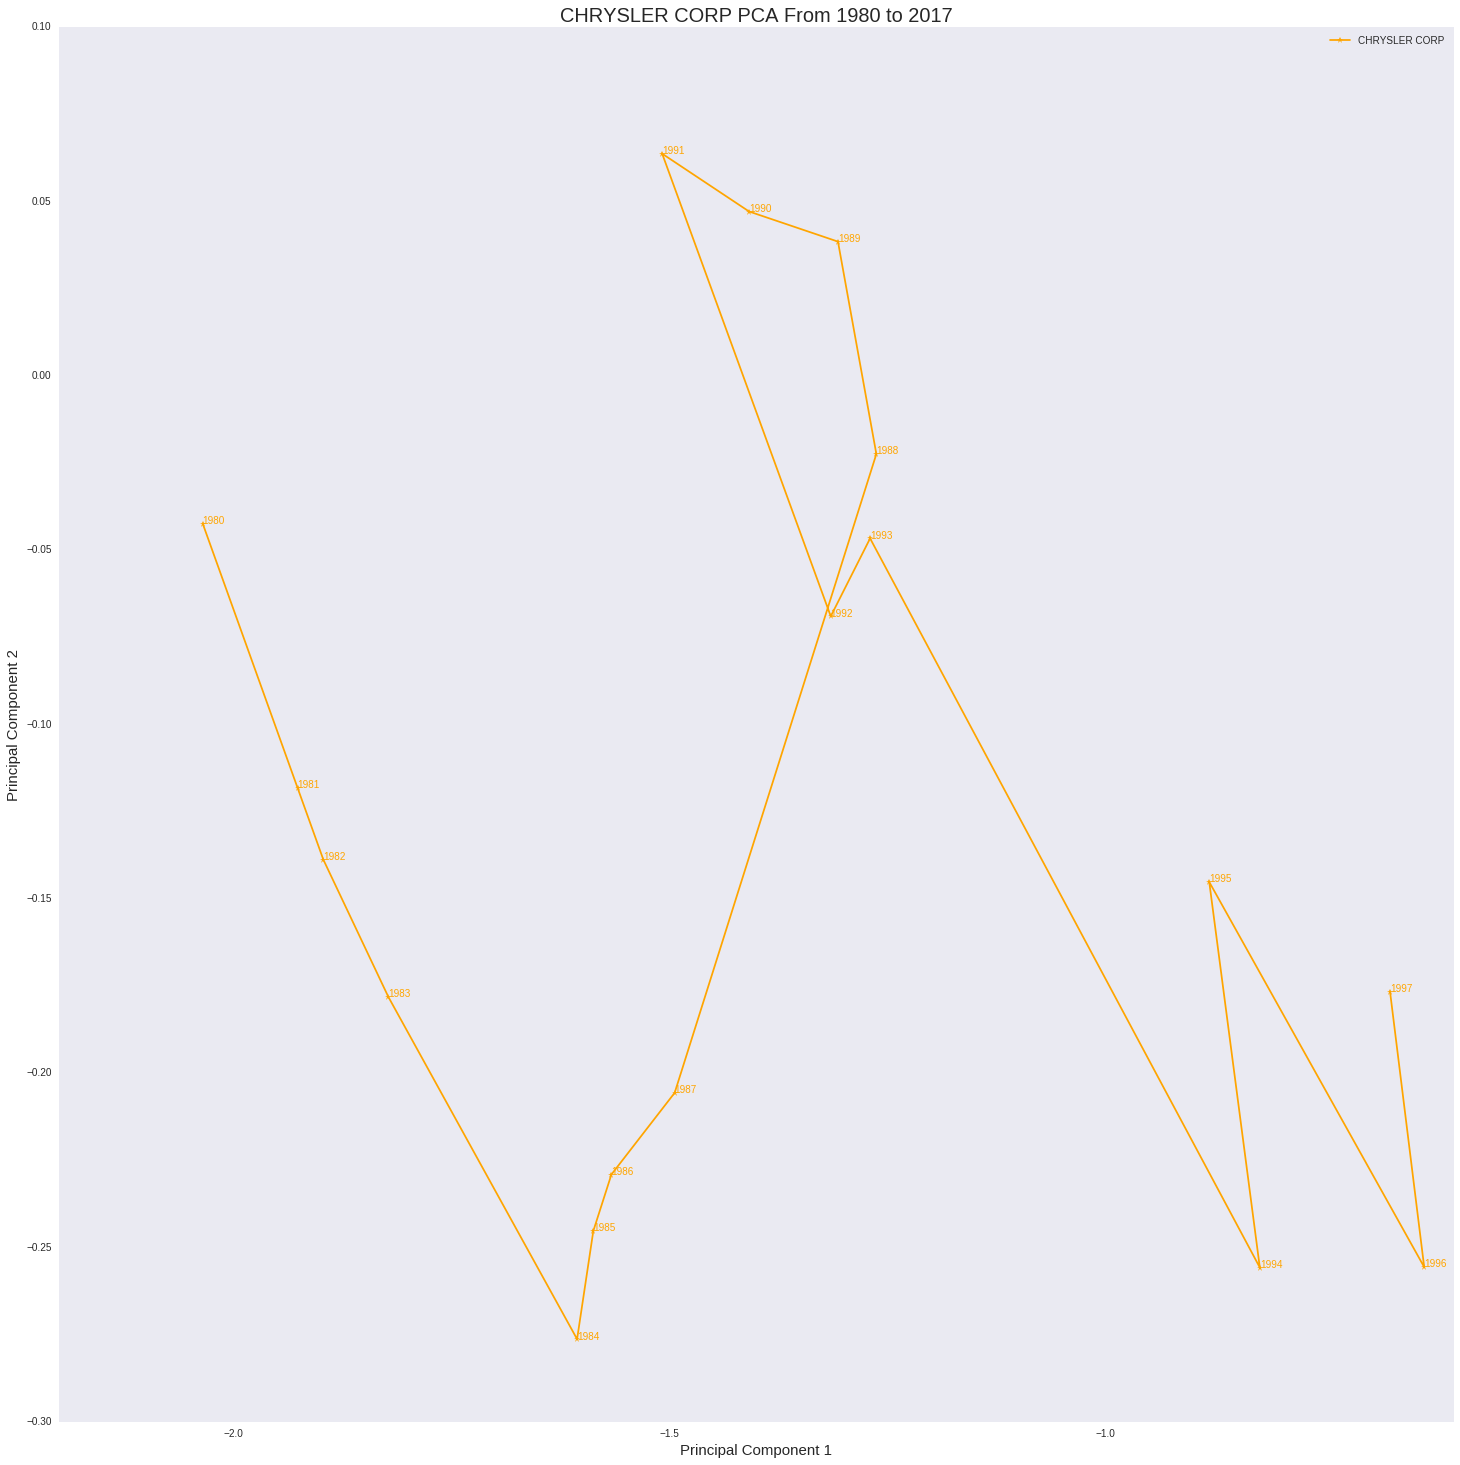
\includegraphics[width=1\textwidth]{./Chrysler}\\[0.1in] \\
\subsection{Ford Motor Co}
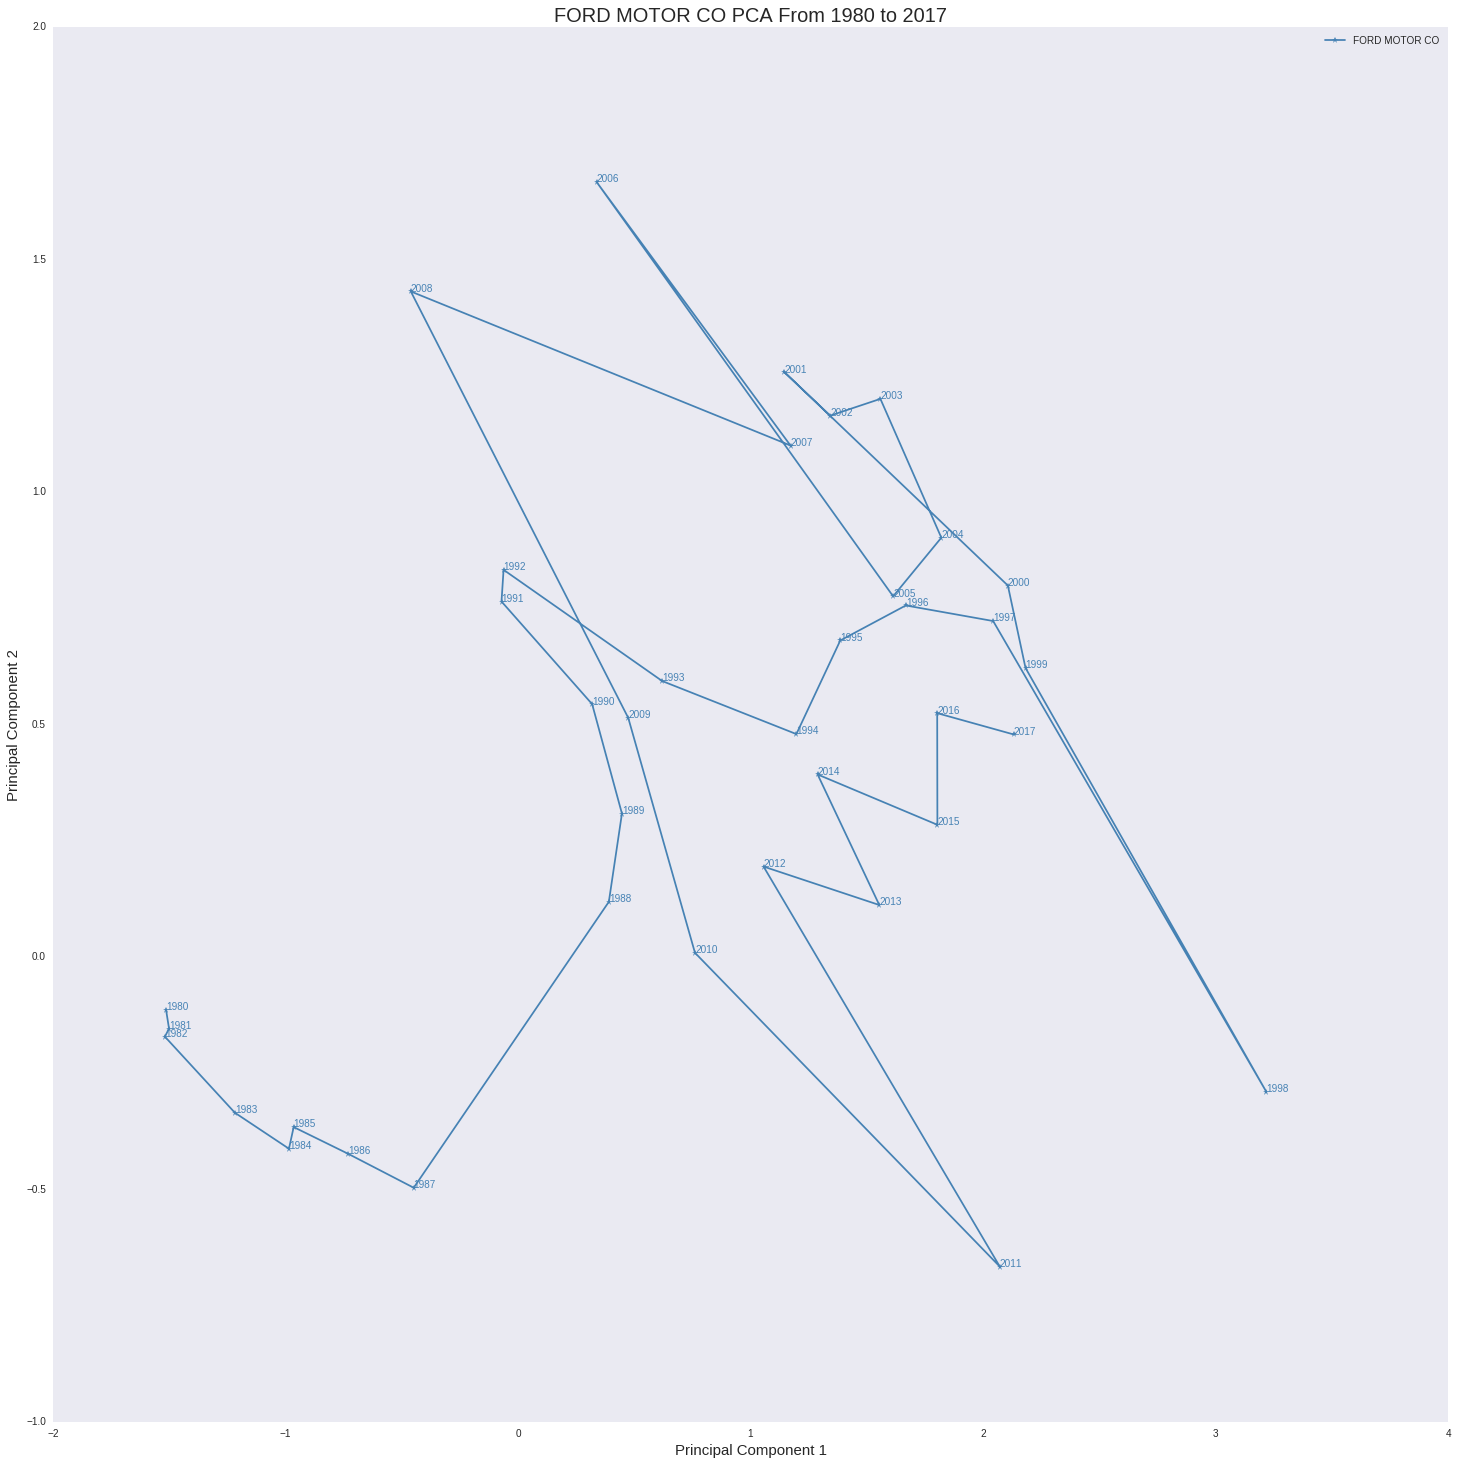
\includegraphics[width=1\textwidth]{./Ford}\\[0.1in] \\
\subsection{General Motors Co}
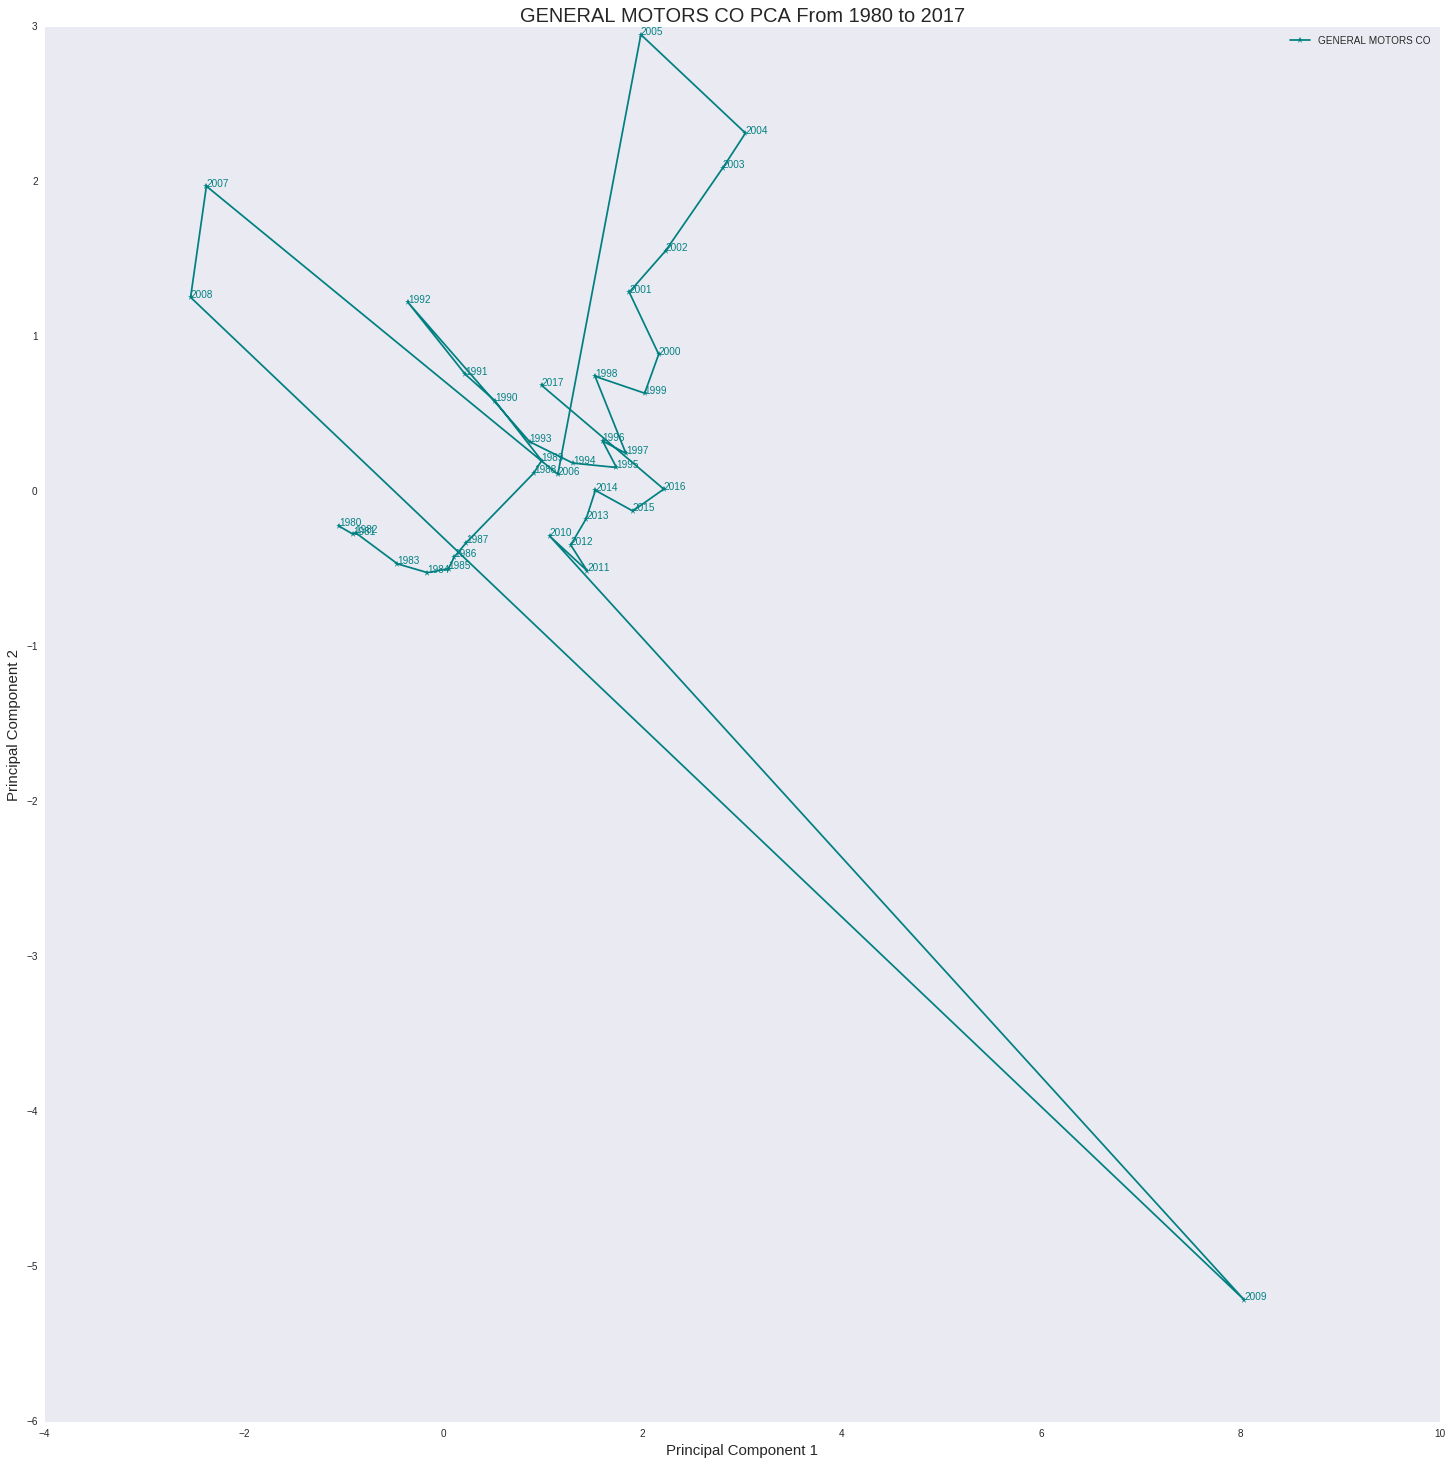
\includegraphics[width=1\textwidth]{./GM}\\[0.1in] \\

\section{Computers}
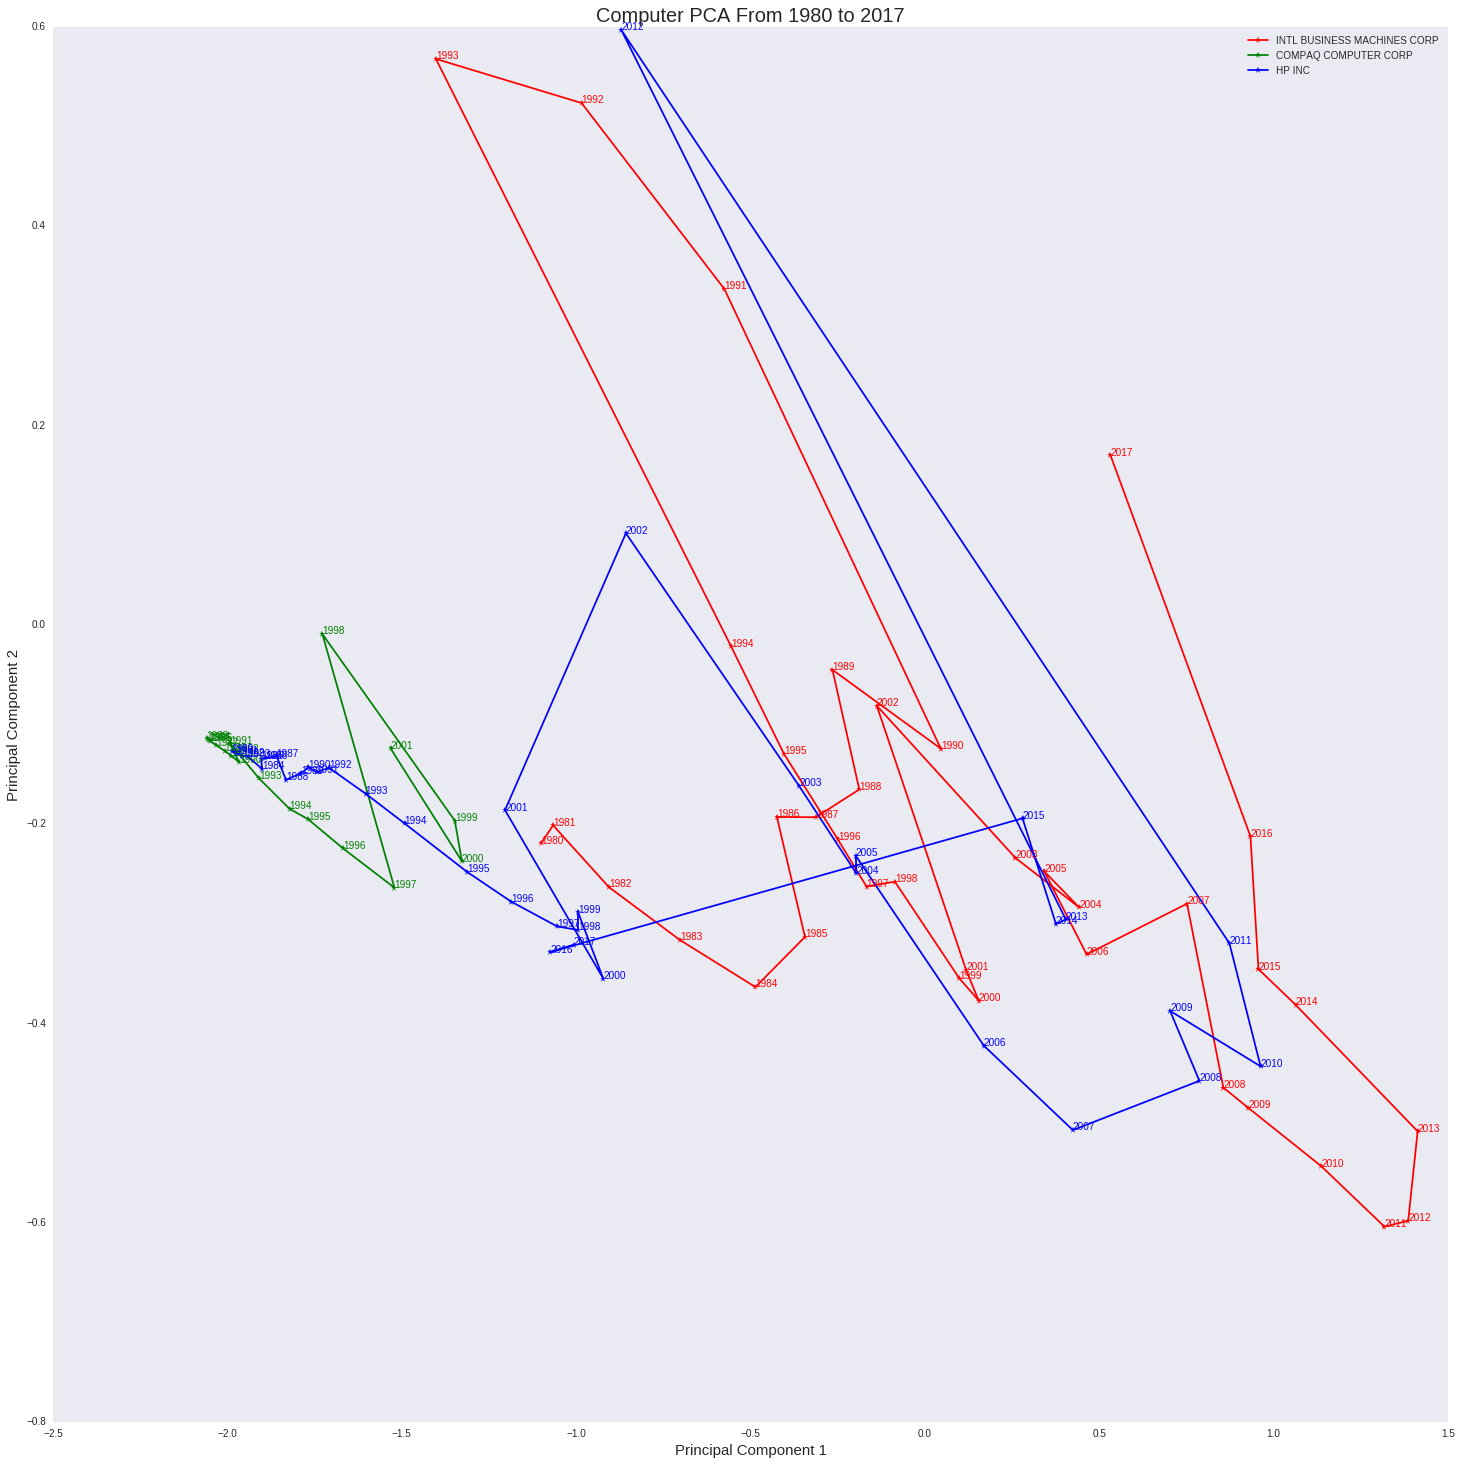
\includegraphics[width=1\textwidth]{./Computers}\\[0.1in] \\
\subsection{HP Inc}
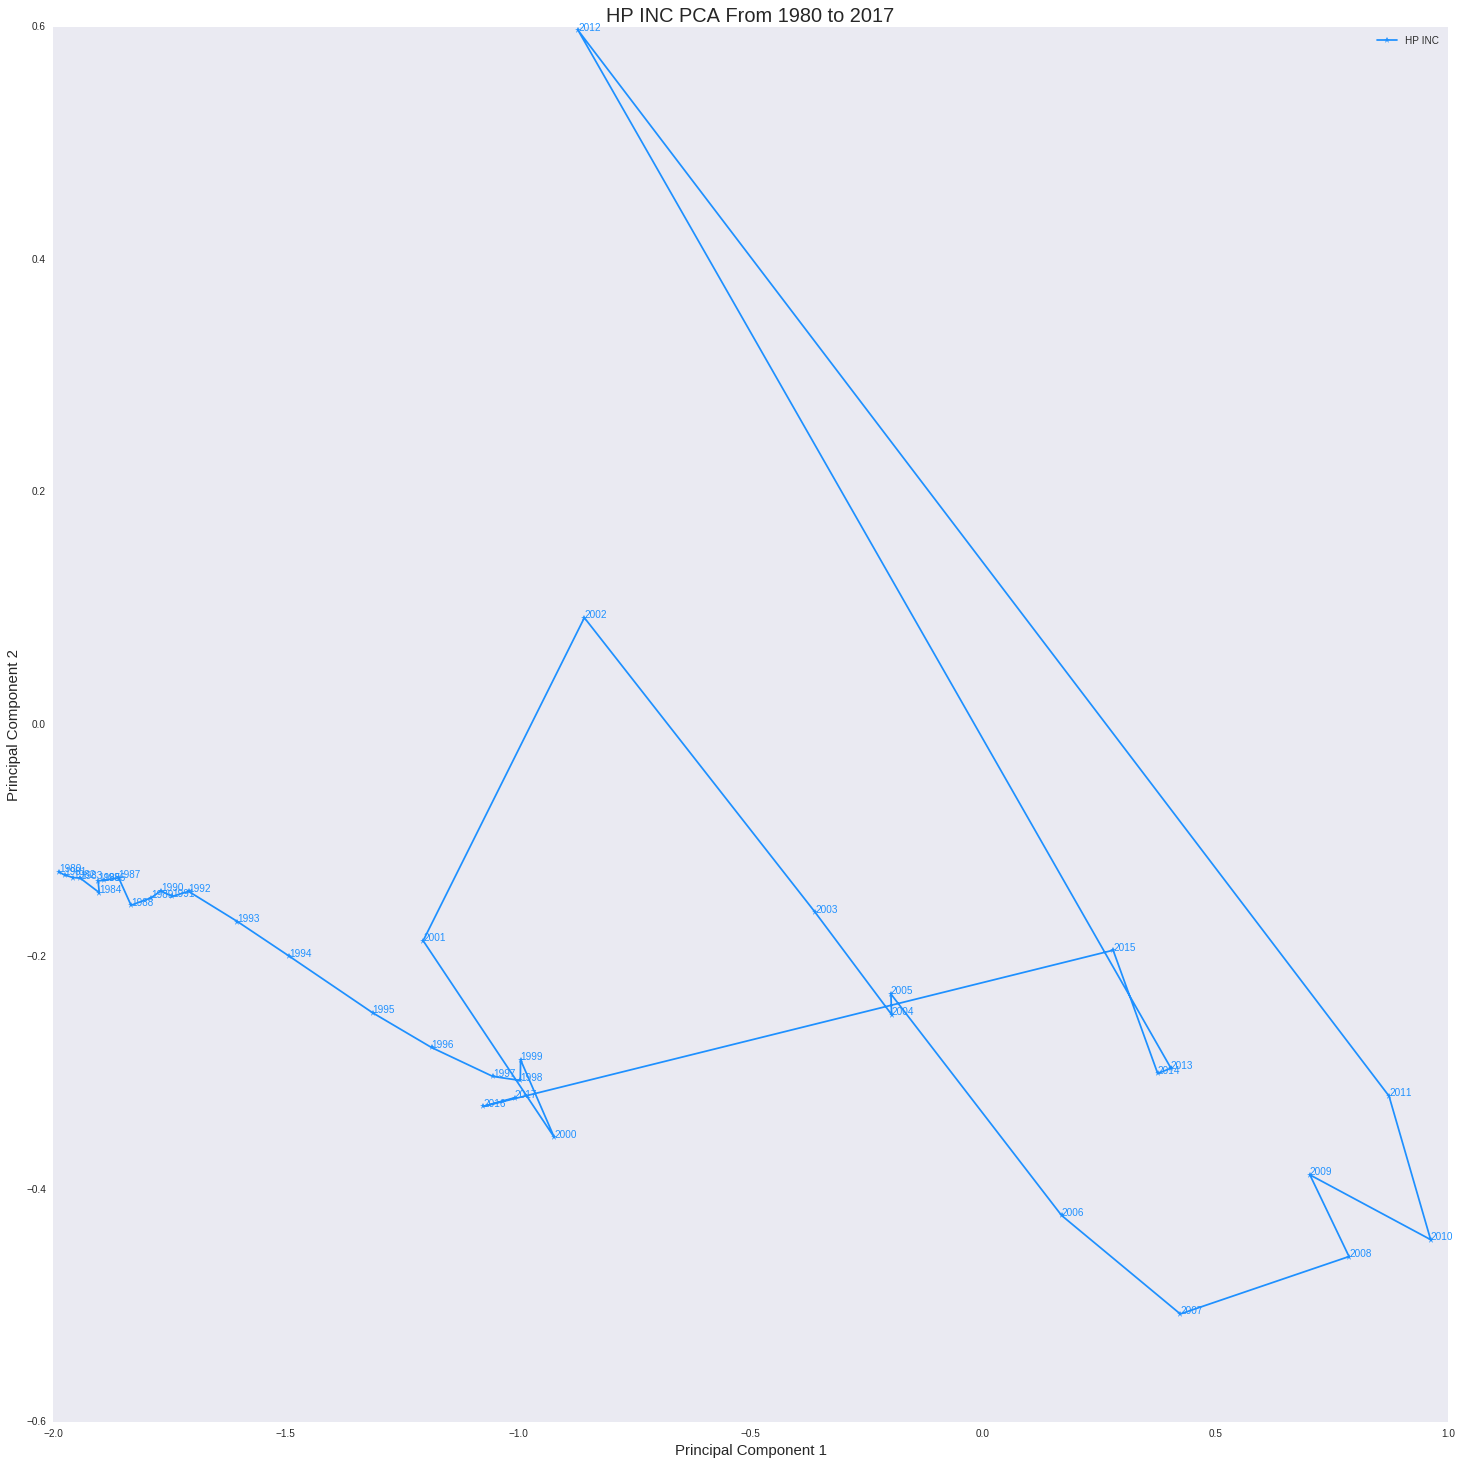
\includegraphics[width=1\textwidth]{./HP}\\[0.1in] \\
\subsection{Compaq Inc}
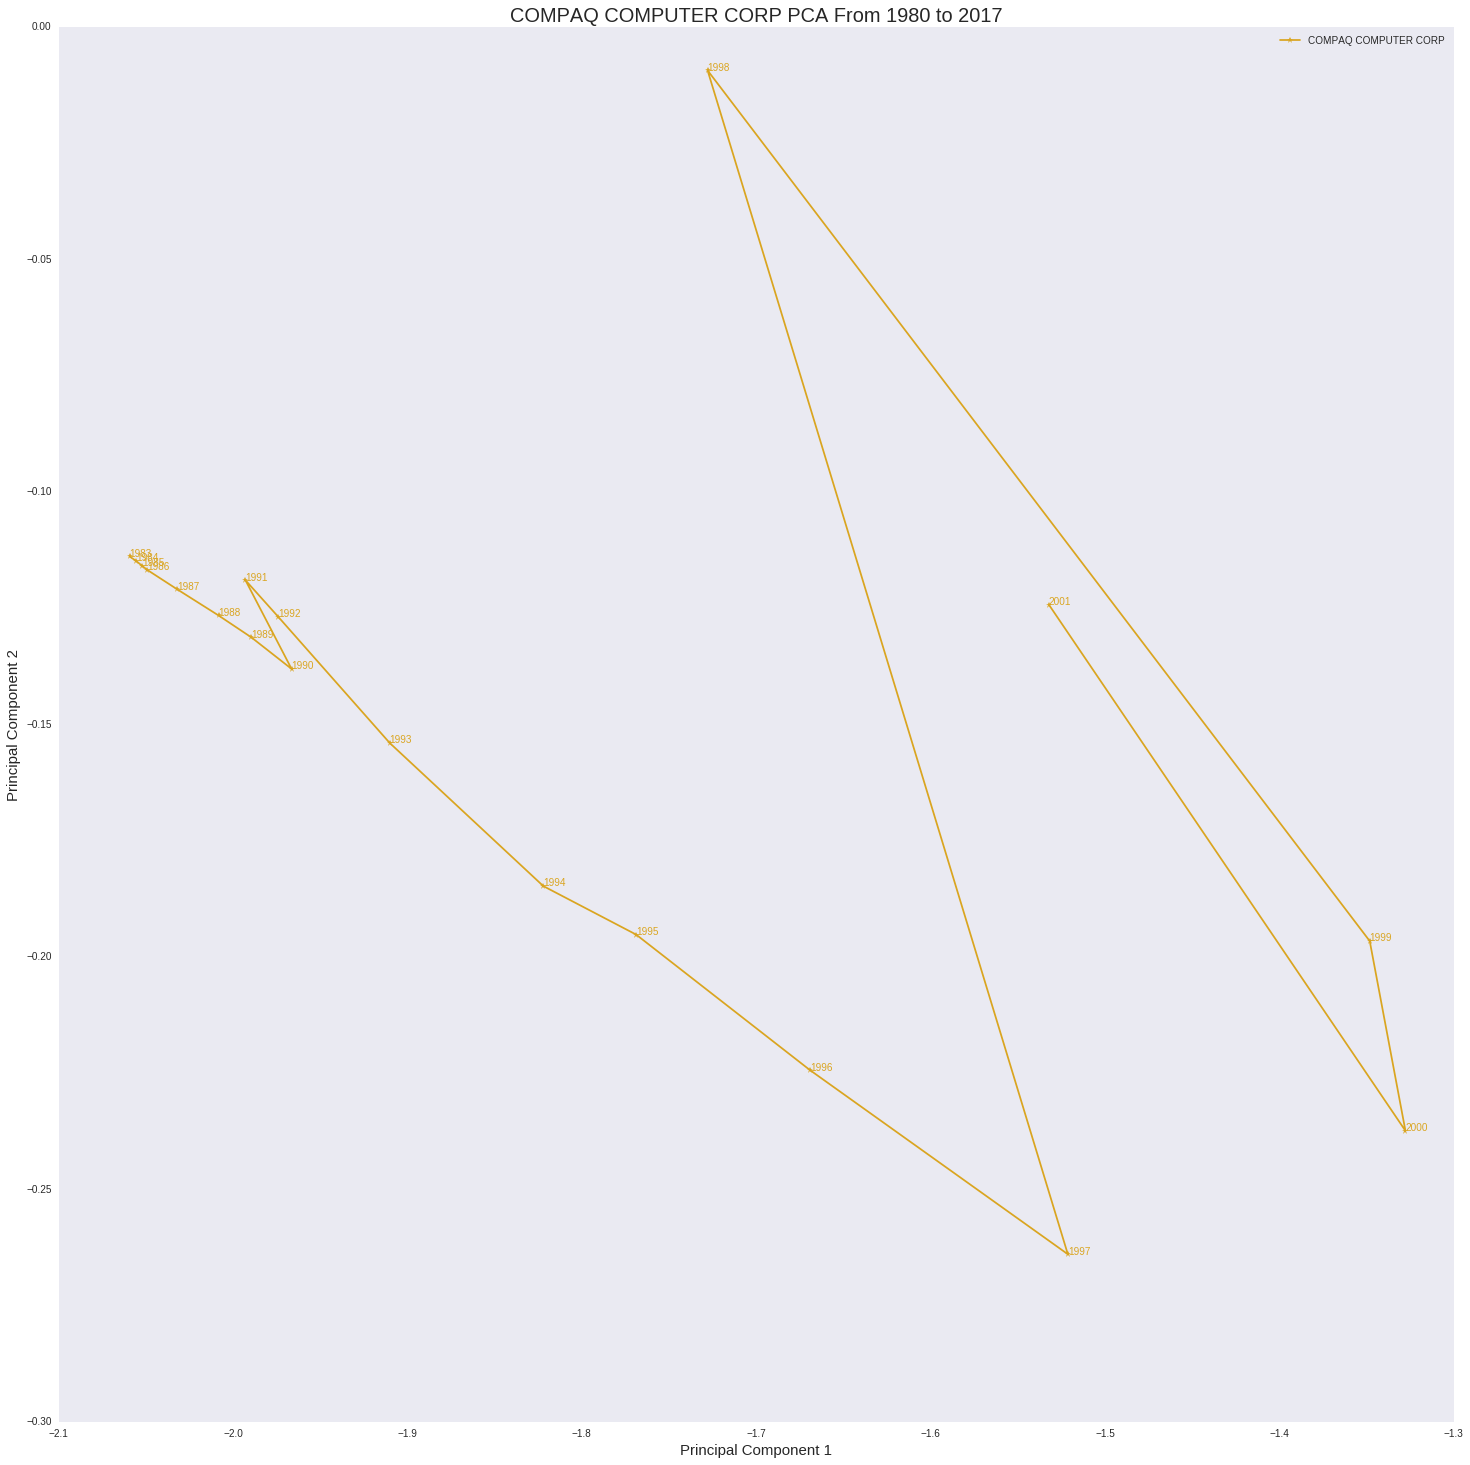
\includegraphics[width=1\textwidth]{./Compaq}\\[0.1in] \\
\subsection{International Business Machines Corp}
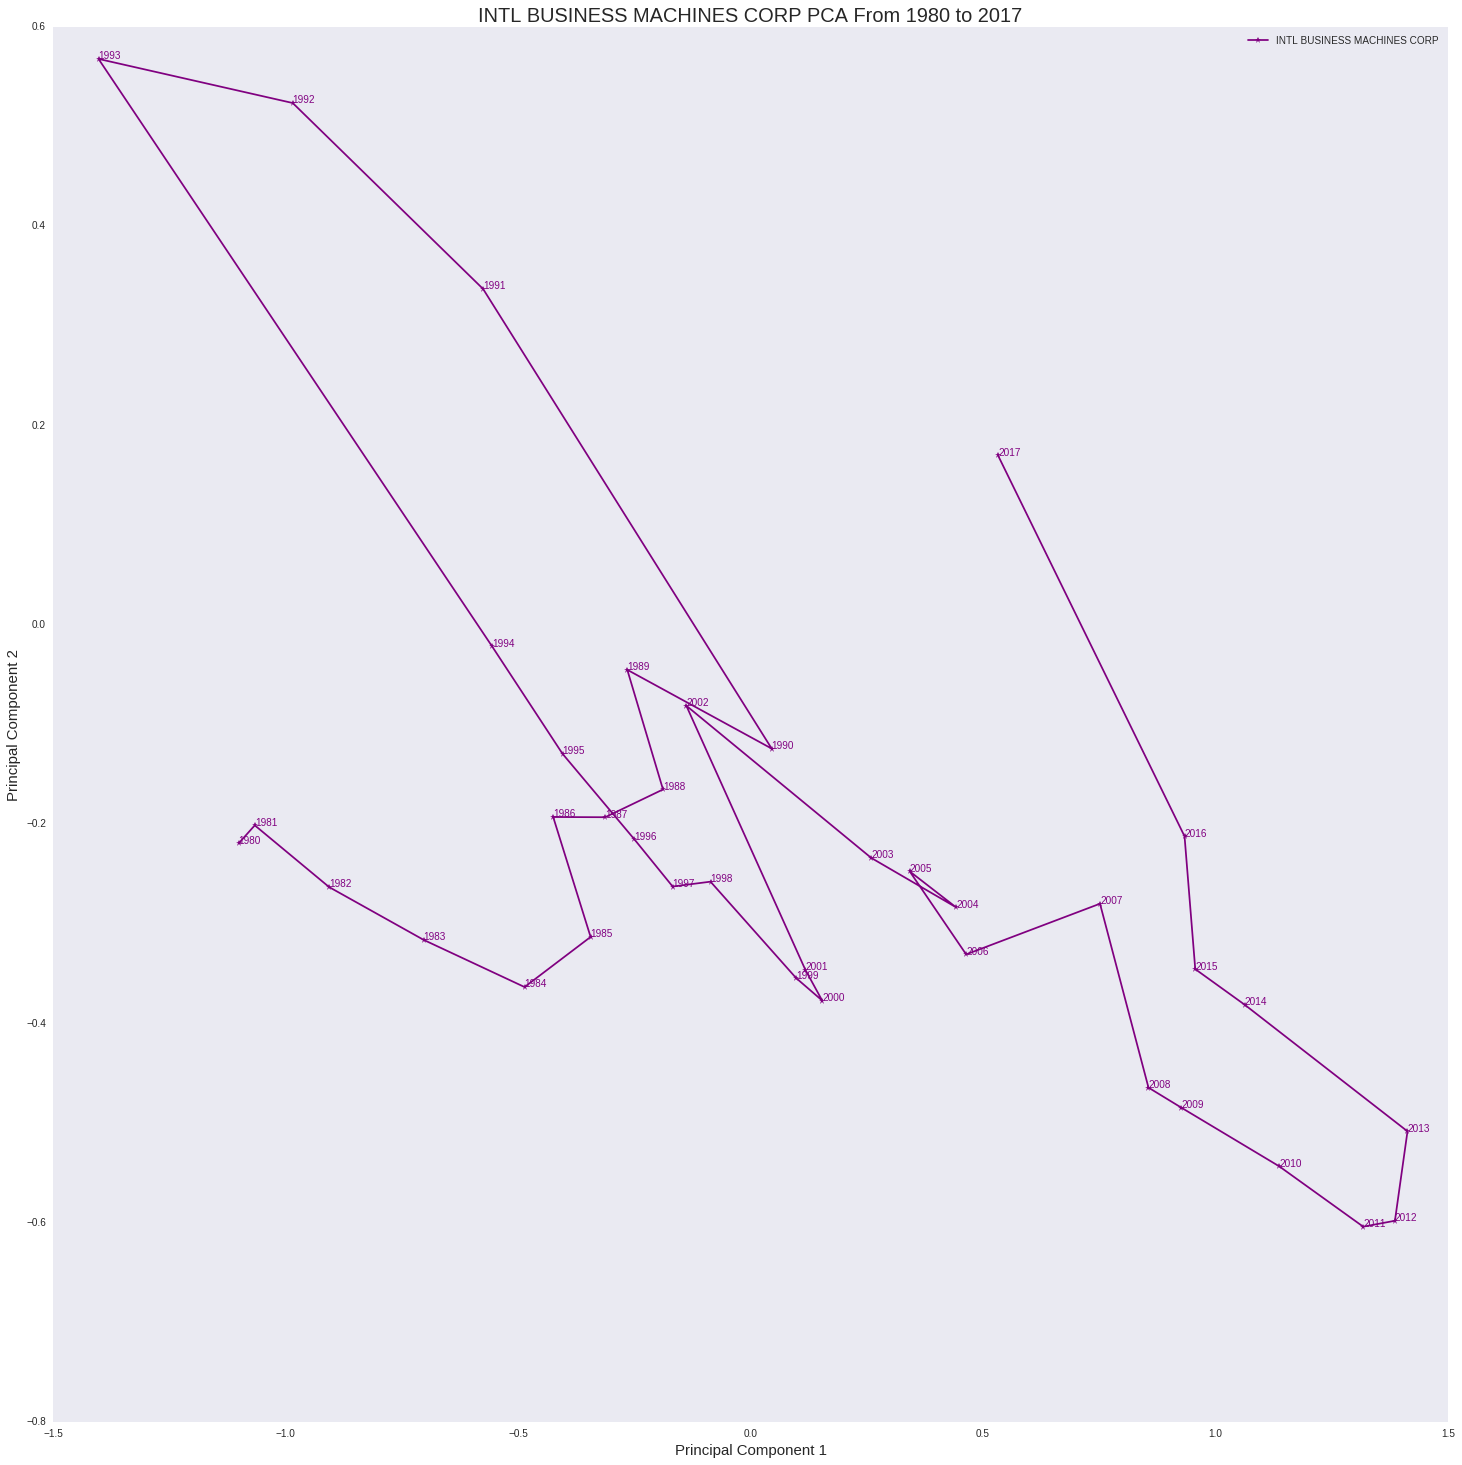
\includegraphics[width=1\textwidth]{./IBM}\\[0.1in] \\
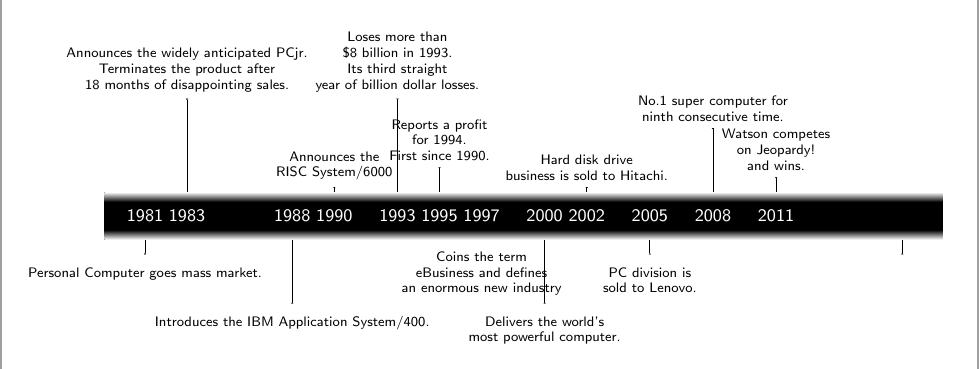
\includegraphics[width=1\textwidth]{./IBMtimeline}\\[0.1in] \\

\section{Telecommunications}
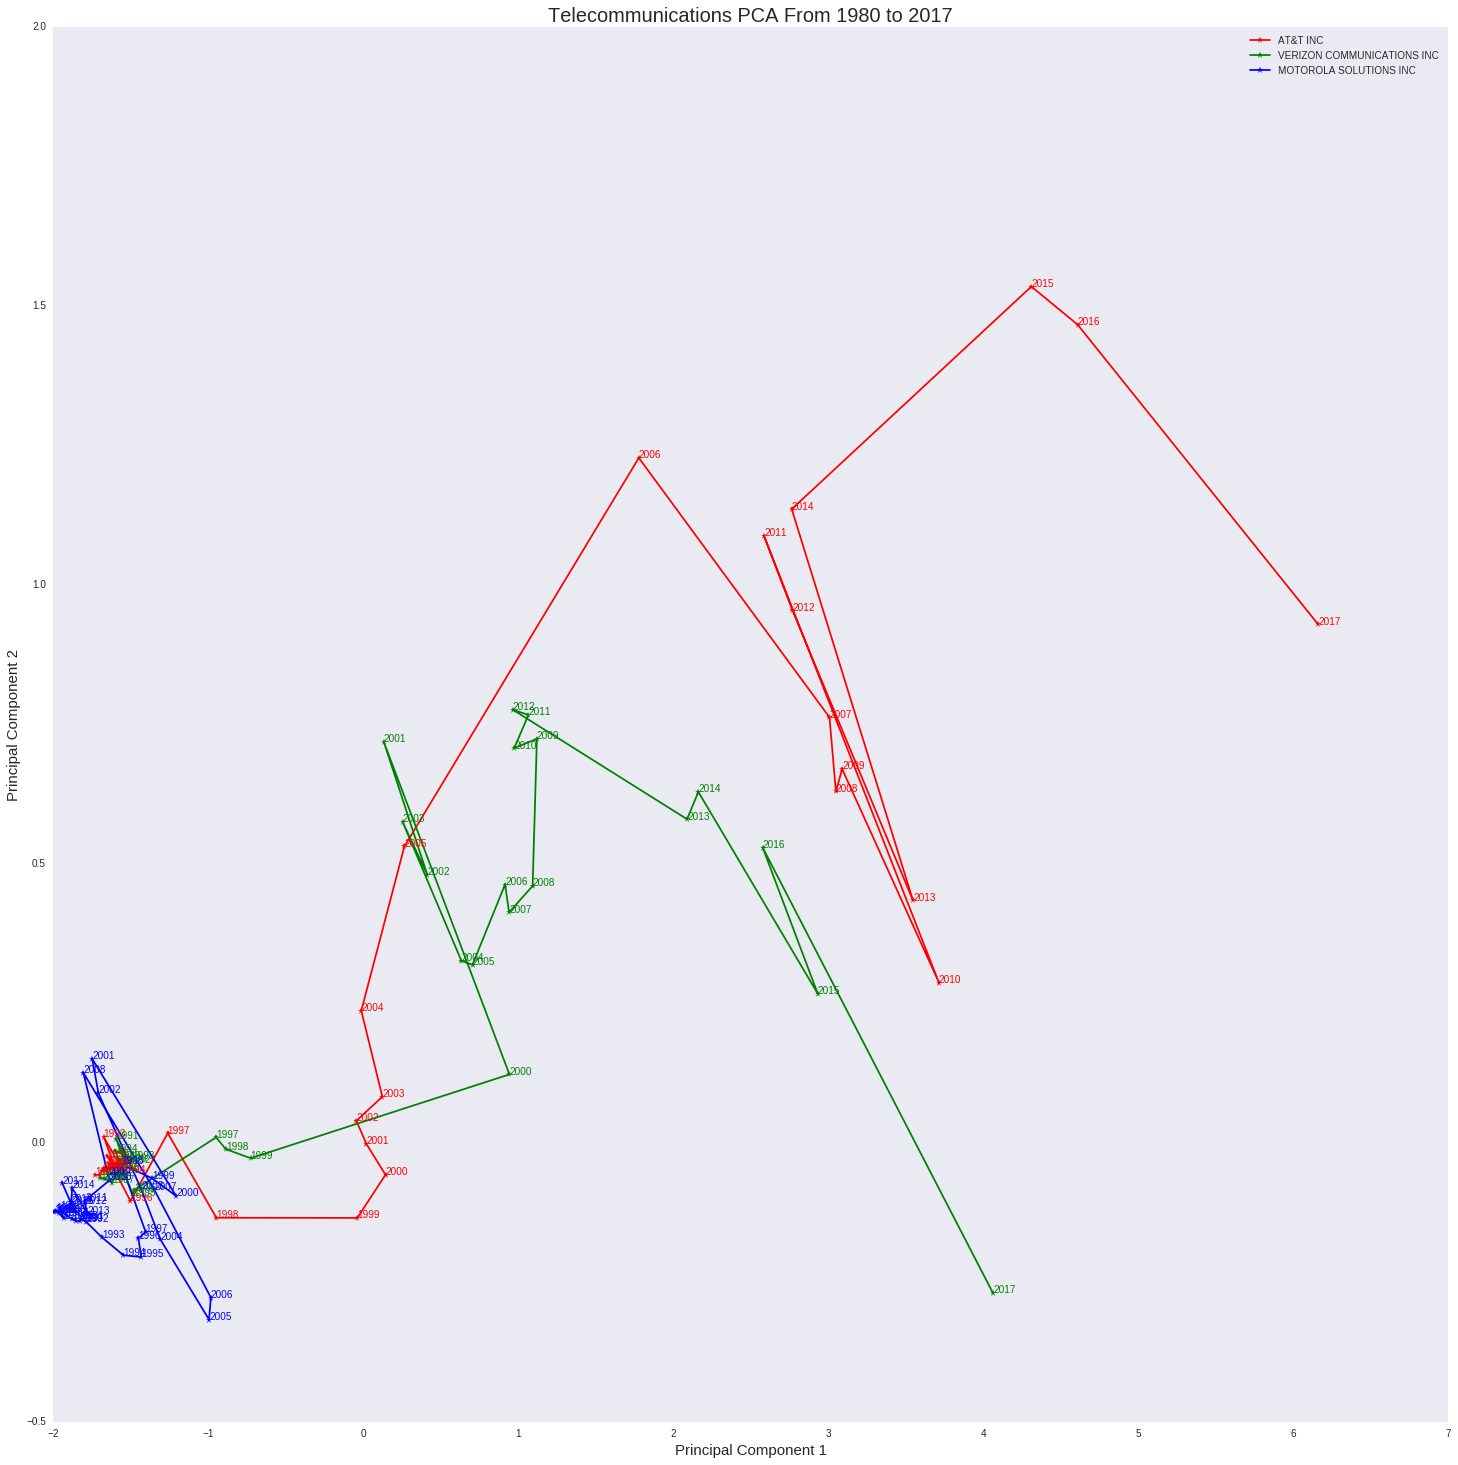
\includegraphics[width=1\textwidth]{./Telecommunications}\\[0.1in] \\
\subsection{Motorola Solutions Inc}
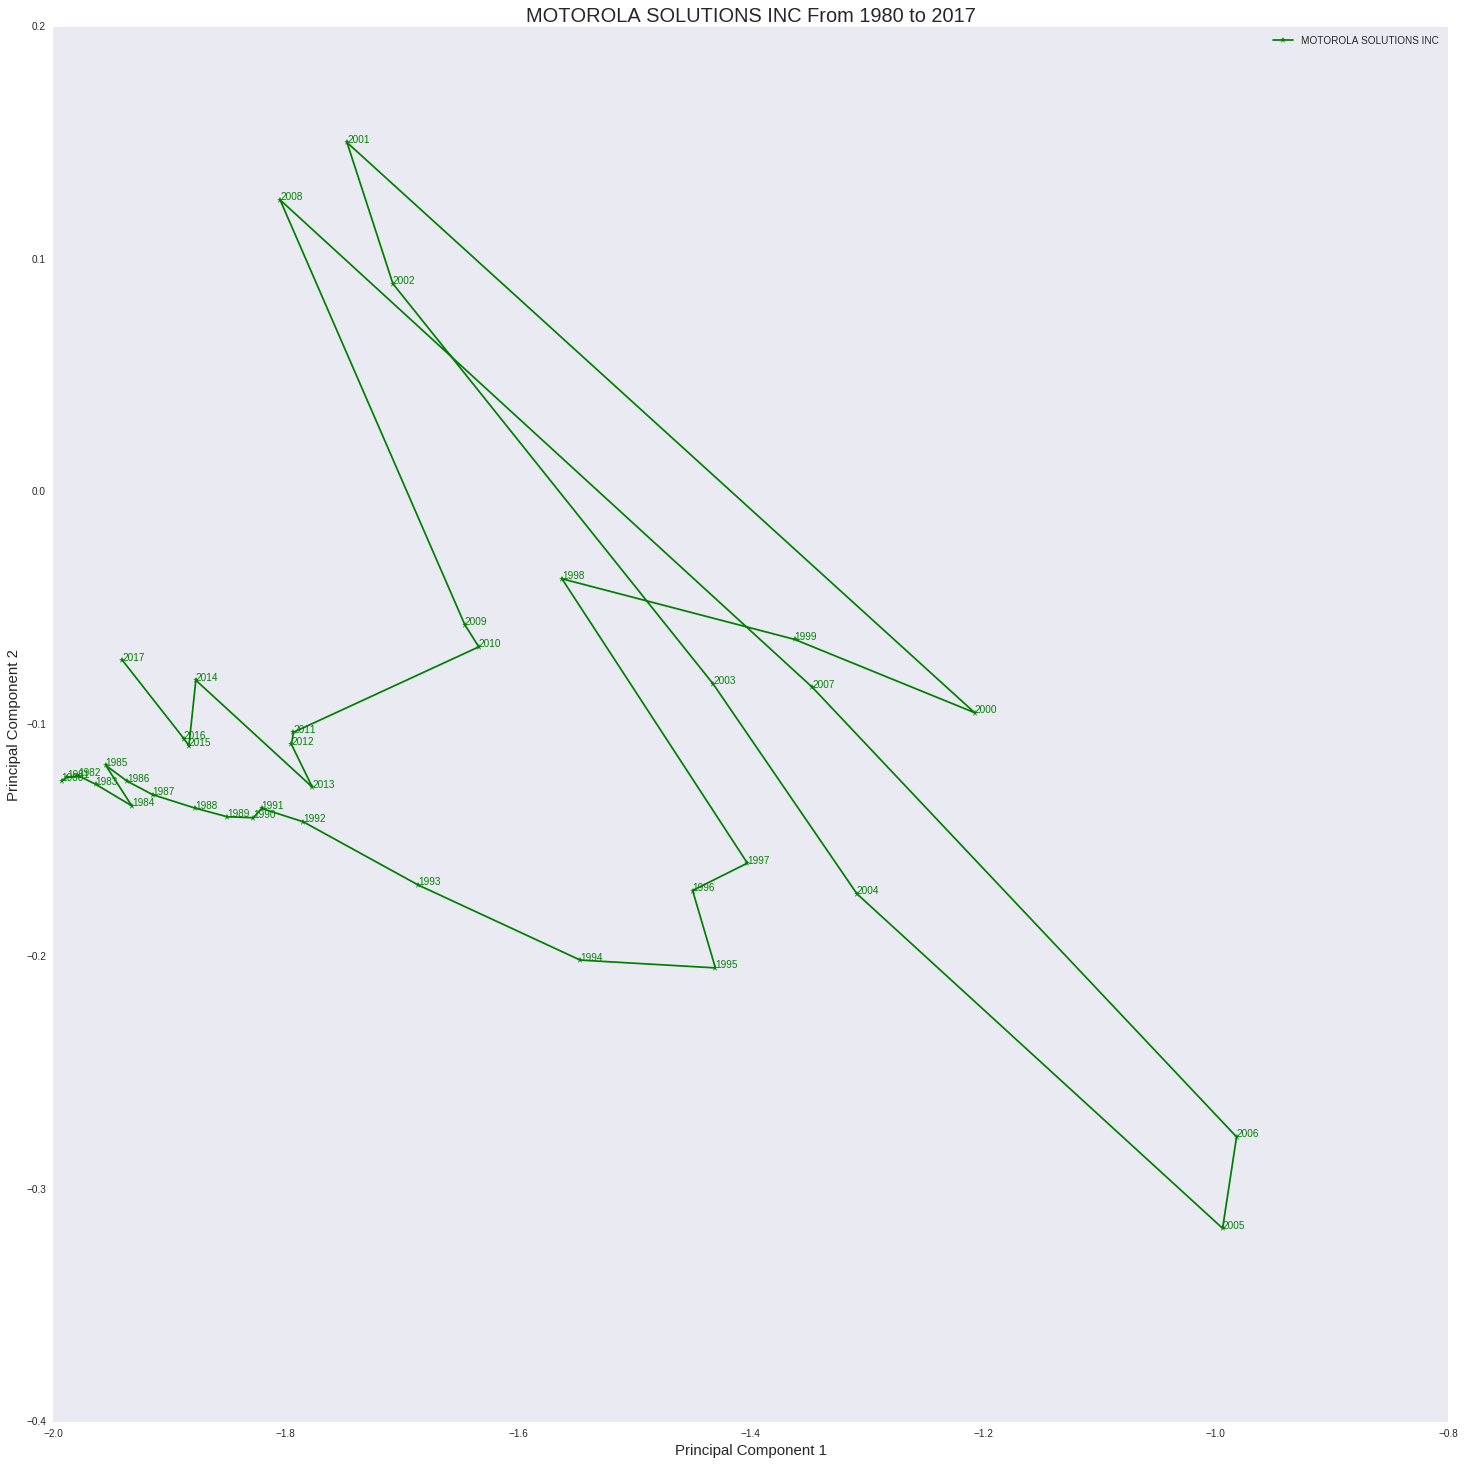
\includegraphics[width=1\textwidth]{./Motorola}\\[0.1in] \\
\subsection{Verizon Communications Inc}
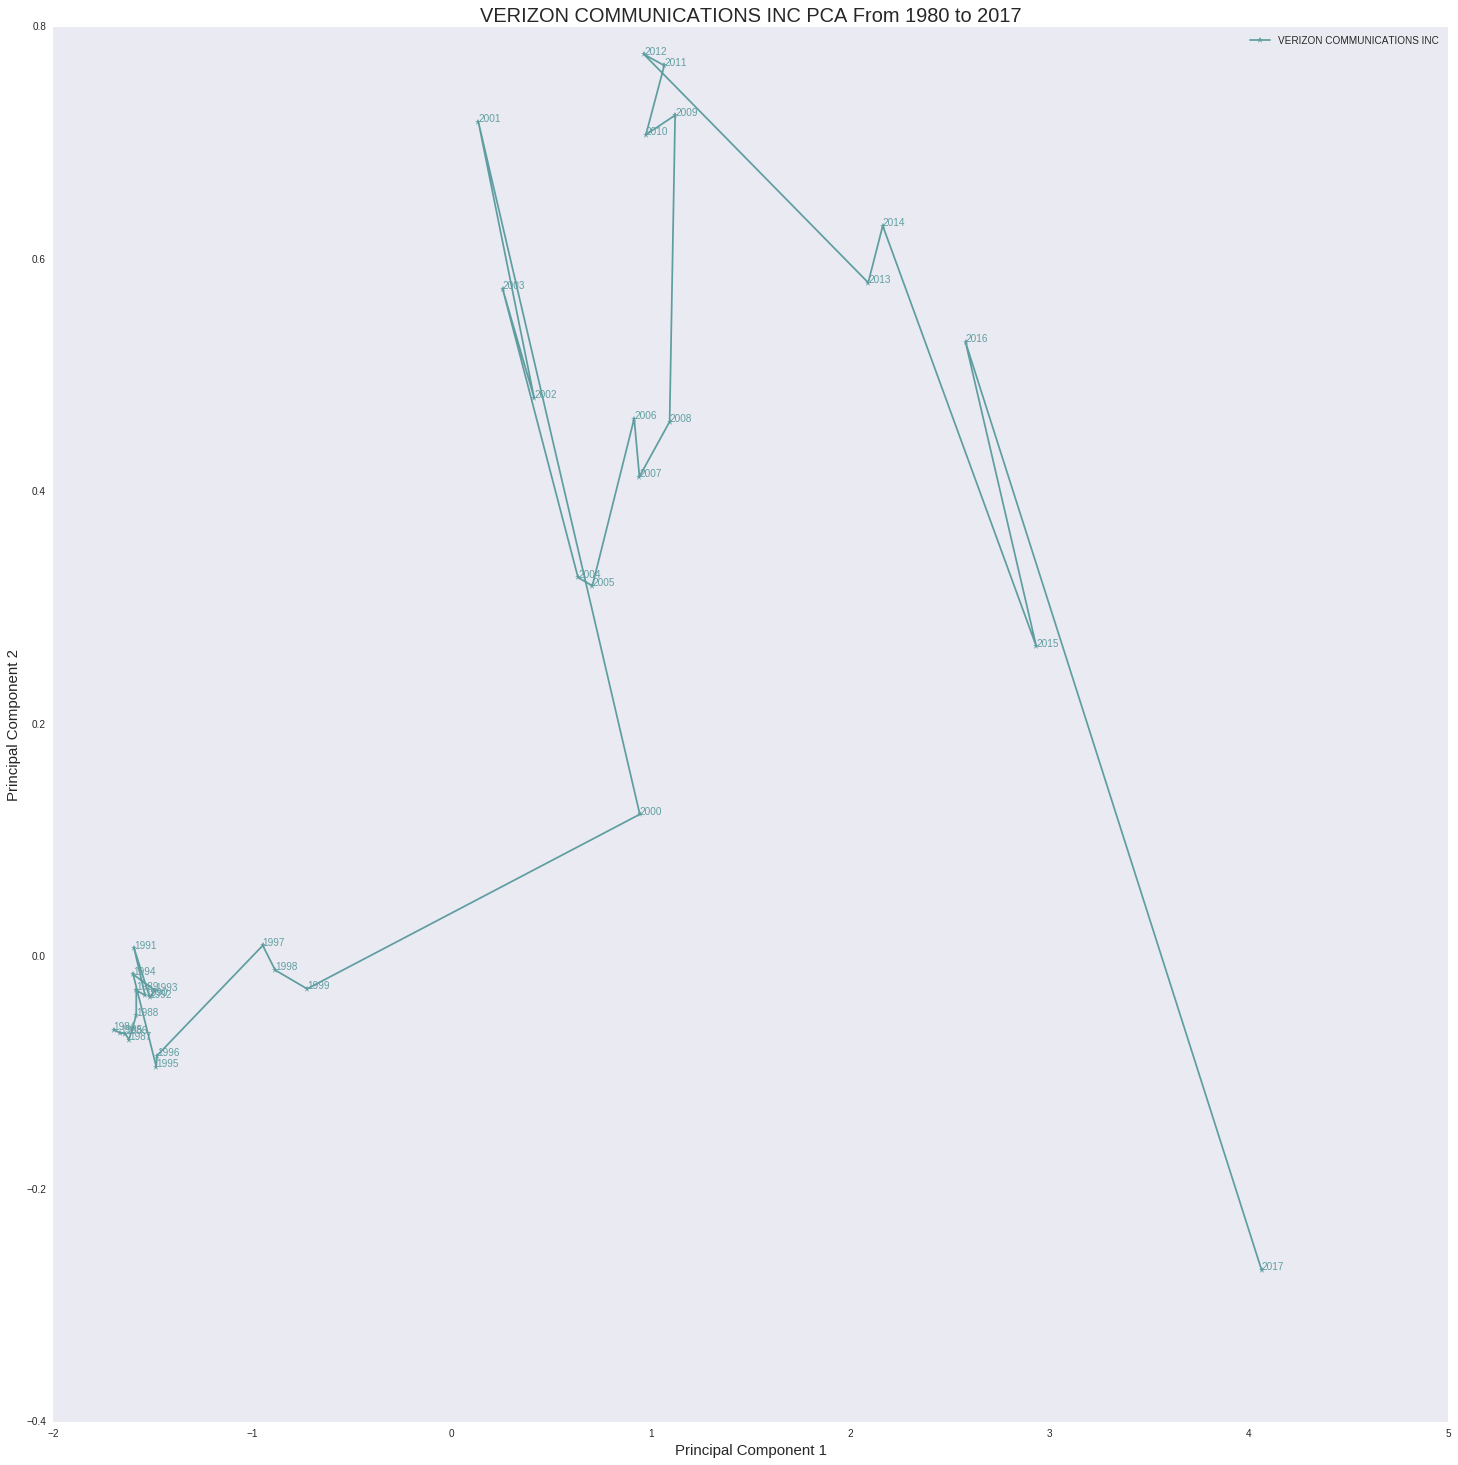
\includegraphics[width=1\textwidth]{./Verizon}\\[0.1in] \\
\subsection{AT\&T Inc}
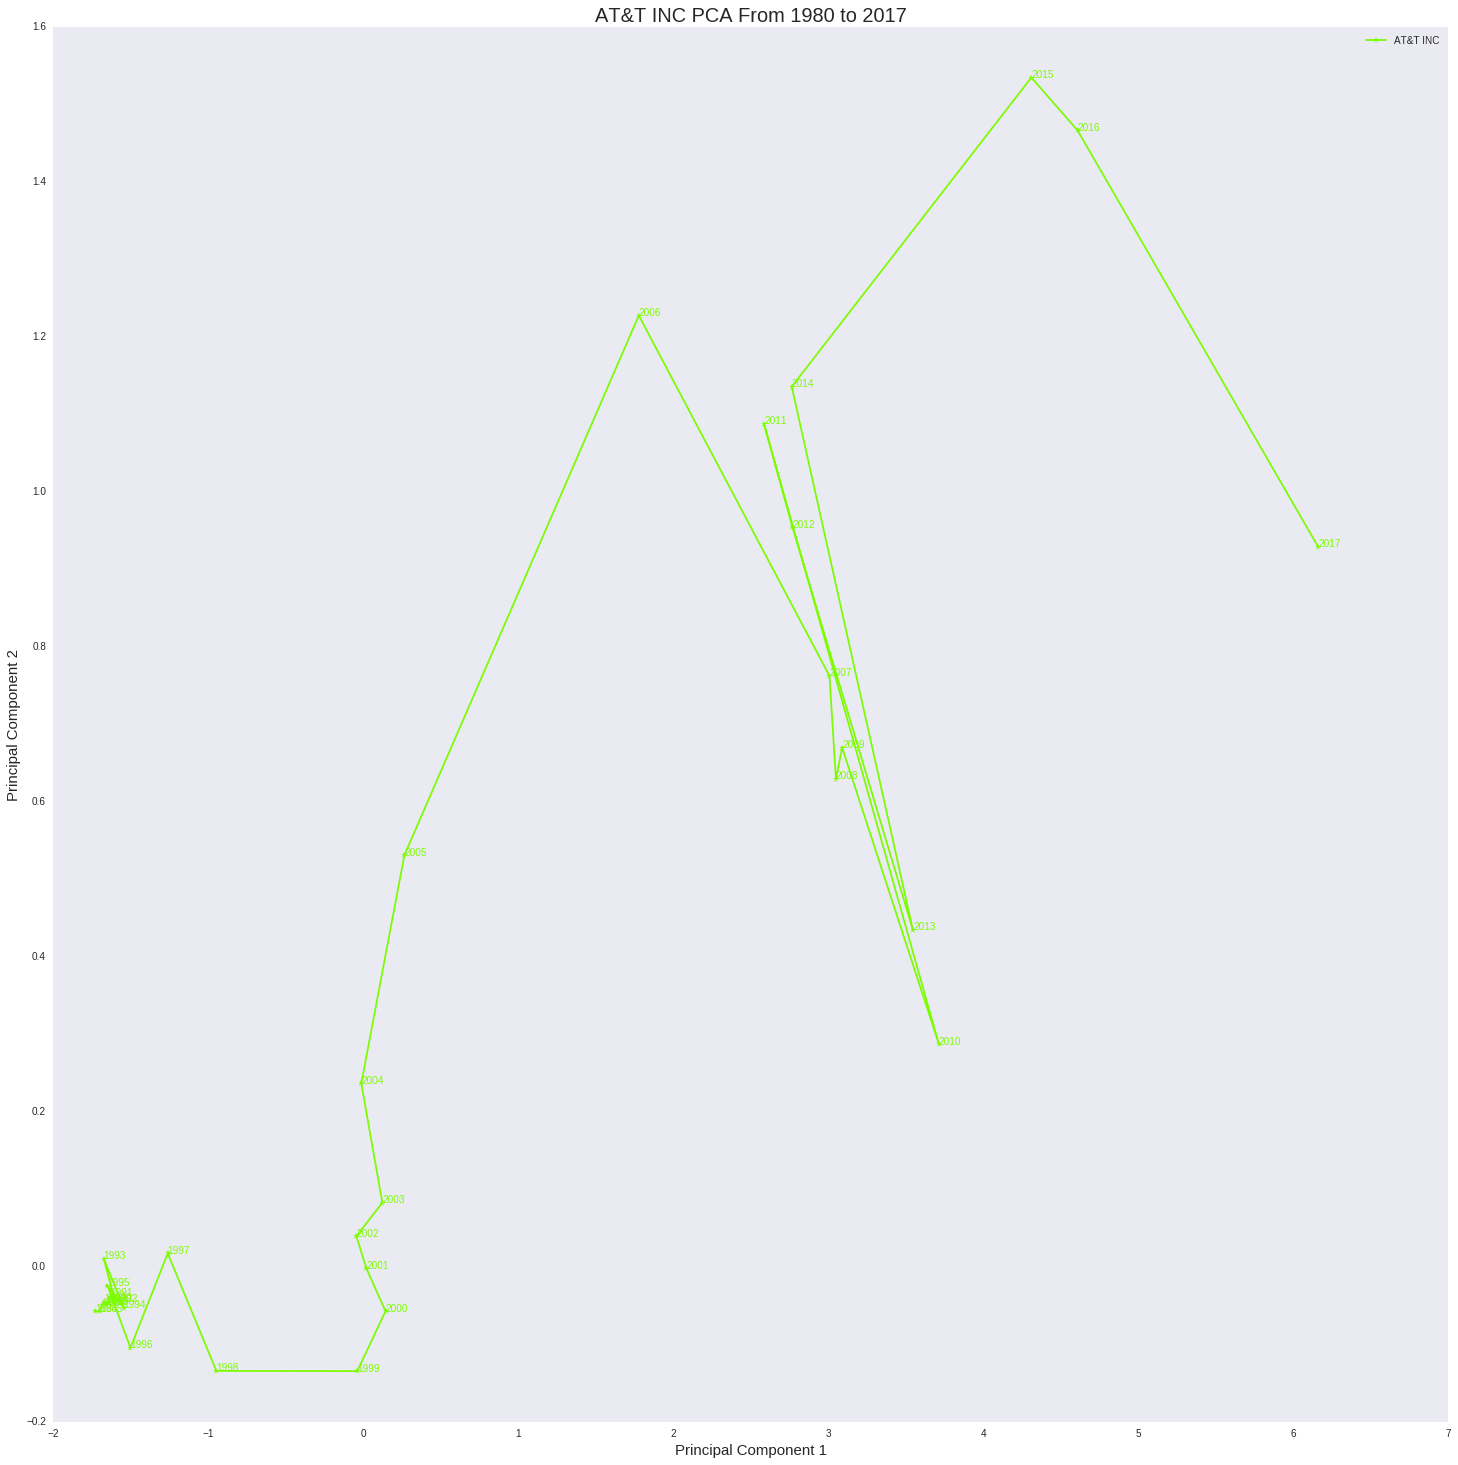
\includegraphics[width=1\textwidth]{./ATT}\\[0.1in] \\

\section{Conglomerate}
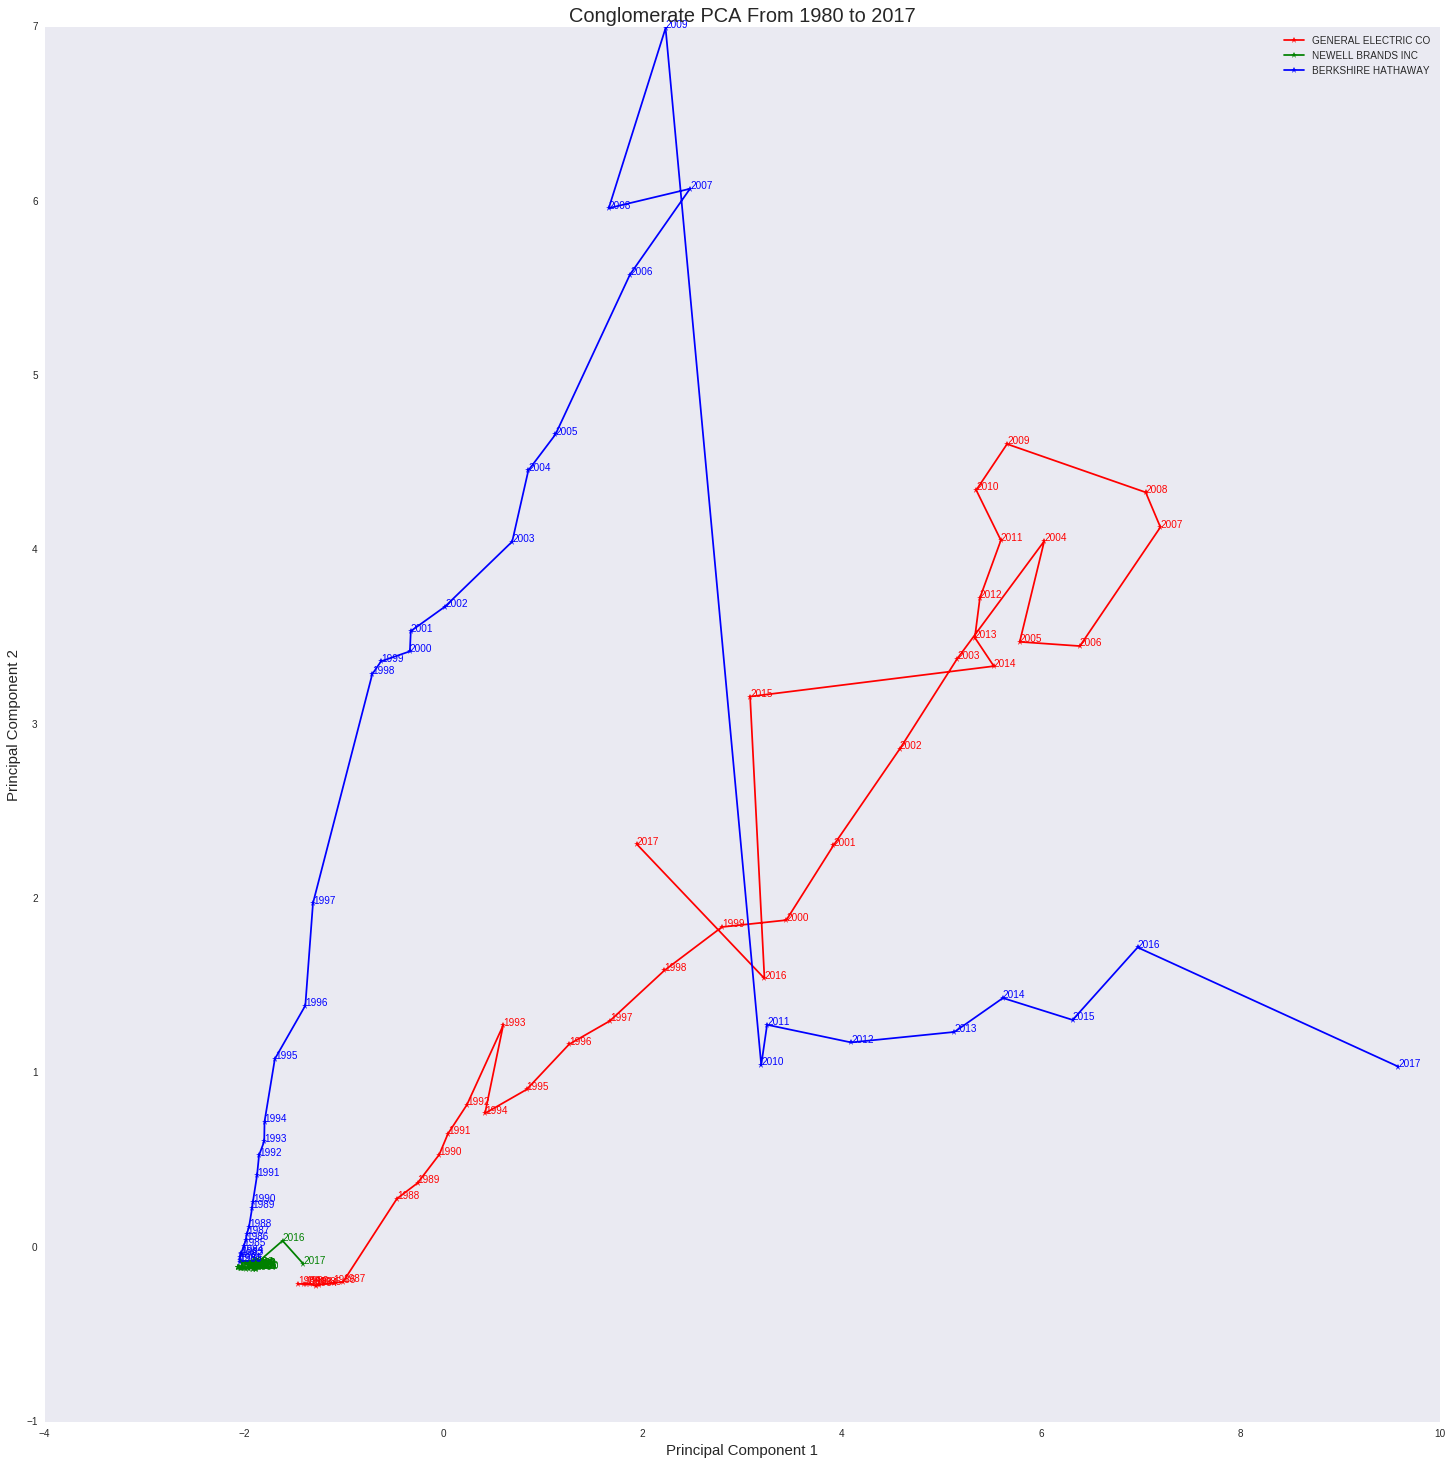
\includegraphics[width=1\textwidth]{./Conglomerates}\\[0.1in] \\
\subsection{Newell Brands Inc}
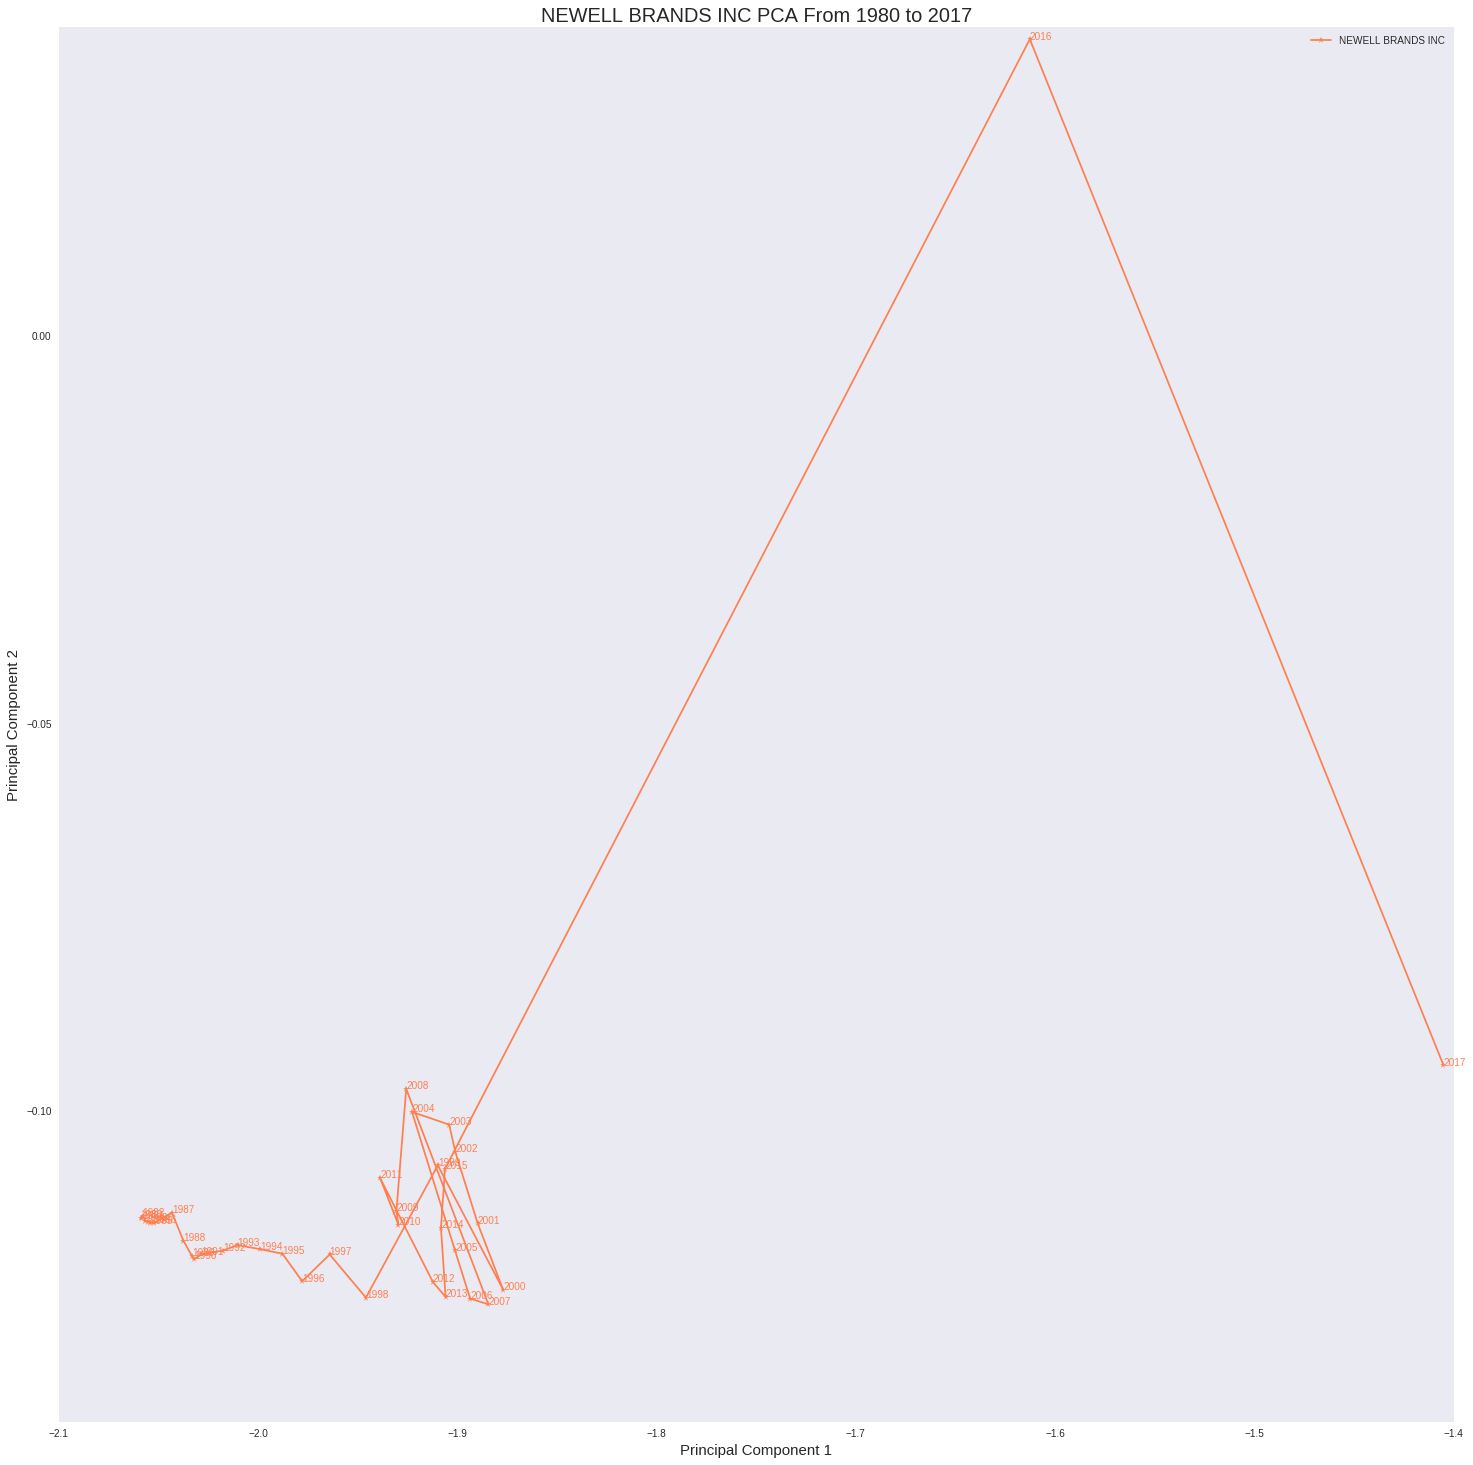
\includegraphics[width=1\textwidth]{./Newell}\\[0.1in] \\
\subsection{General Electric Co}
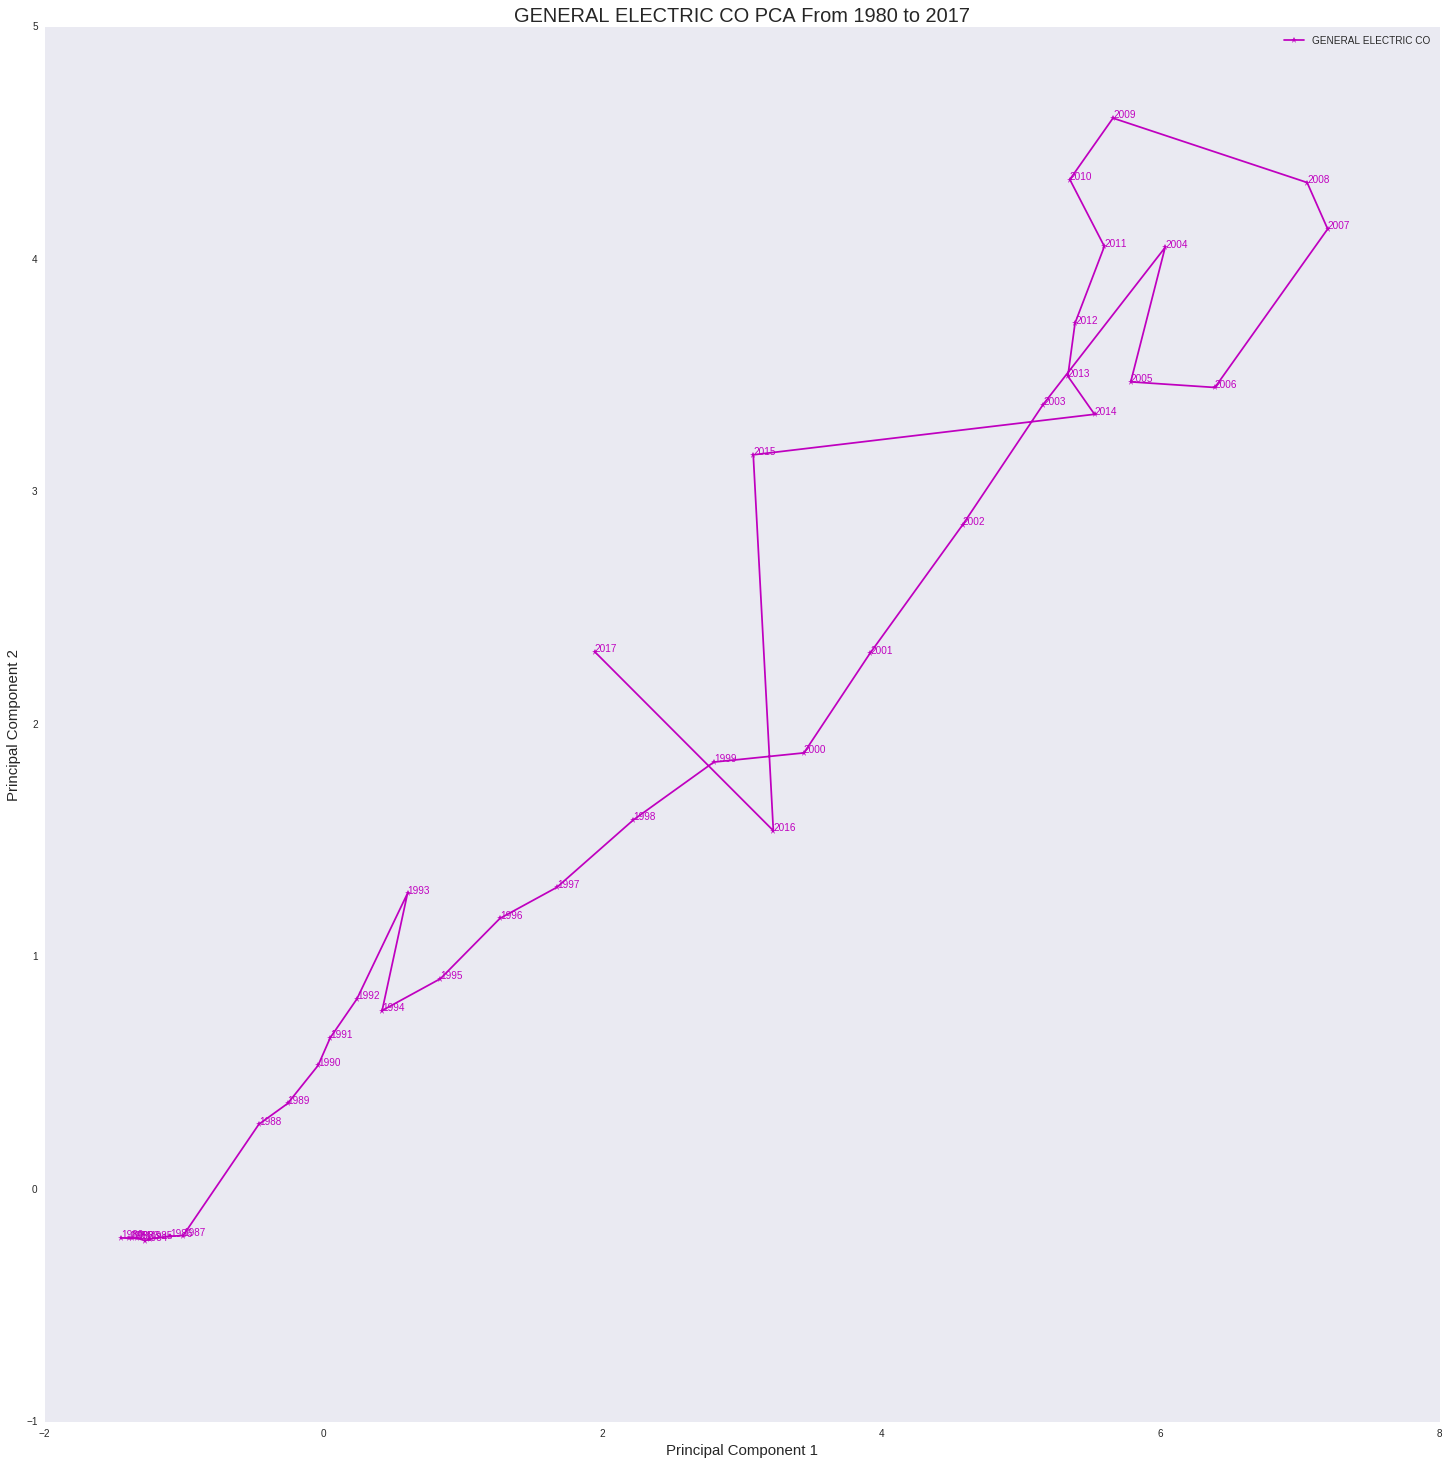
\includegraphics[width=1\textwidth]{./GE}\\[0.1in] \\
\subsection{Berkshire Hathaway}
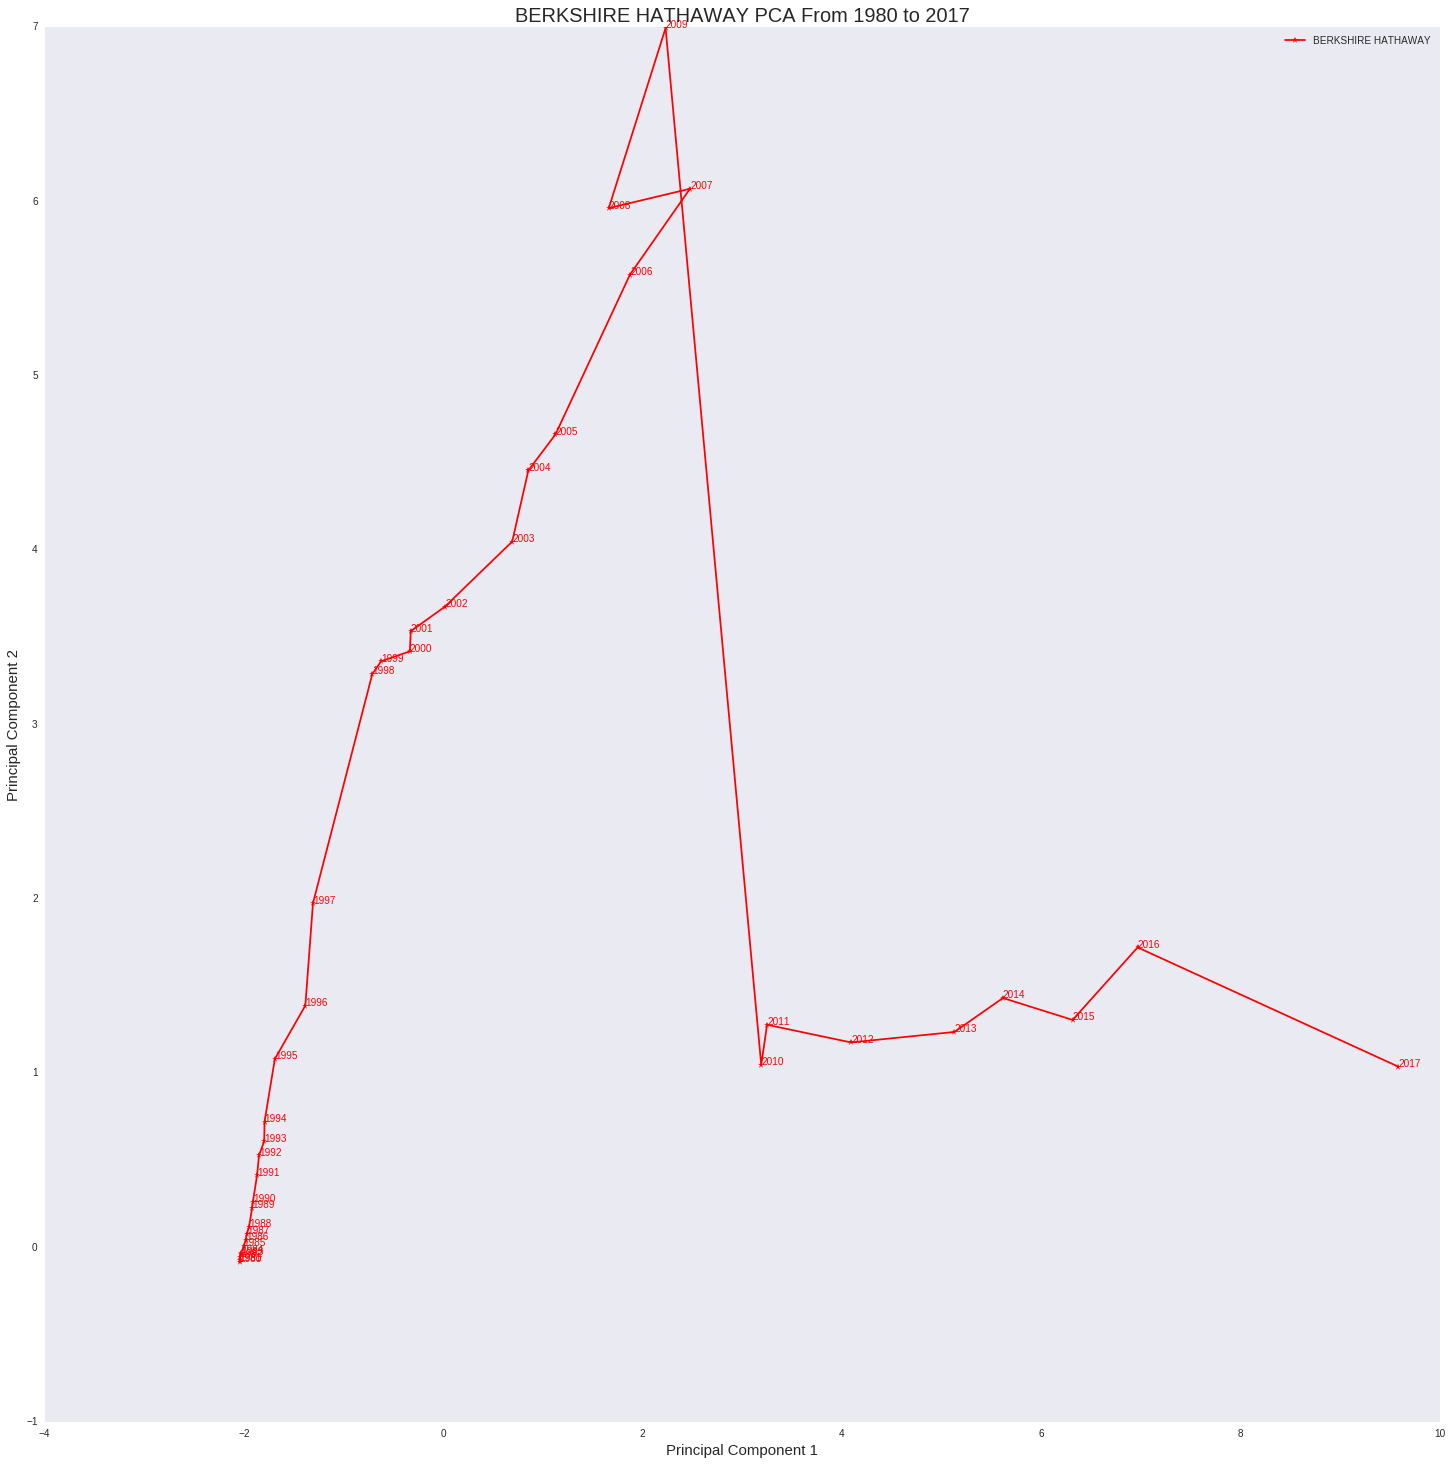
\includegraphics[width=1\textwidth]{./Berkshire_Hathaway}\\[0.1in] \\
\chapter{Conclusion}



	From the beginning of this project, the intent has been to understand how plausible it would be to determine if there are predictable market forces acting within a given industry. The continued recurrence of the same highly connected companies implies the market forces that govern these few companies in turn govern their respective industries. Through the PCA reduction of several variables the graphs constructed have given great insight into how these forces can sway even the largest companies over the years. From the housing market affecting the hardware industry, to near identical movements within the oil industry and to delayed tough near mirroring moves in the automotive industry.\\
\newline

	These various phenomena within each graph can all be attributed to a major event affect each company. From an acquisition that went well or poorly to an unexpected and expensive recall each change in trajectory has a tangible meaning. These finding give credit to the next phase of this research.\\
\newline

	The next goal for this research into industry force is to move from a descriptive model to a predictive one.  The scope of the study will eventually be expanded to include more companies to build a predictive model. Ideally the model, given a change in trajectory, will be able to predict what the next points in the graph will be. With enough predictions of companies in a given industry it may be possible to determine in what direction an industry and its respective companies will be moving.\\
\newline


\cleardoublepage
%\pagebreak
\phantomsection
\addcontentsline{toc}{chapter}{References}
\begin{thebibliography}{99}

\bibitem{citation-1-name-here}<Name of the reference here>,\ \url{<url here>}

\bibitem{citation-2-name-here}<Name of the reference here>,\ \url{<url here>}

\end{thebibliography}


\end{document}
